\chapter{Camera and \acs{lidar} Calibration}
\label{chapter:calibration}

The focus of this chapter is to detail the considerations and procedures used on sensory calibration, starting by describing the experimental setup. Then, the method used to calibrate the camera and \ac{lidar} intrinsic parameters are detailed and results are shown. After proper calibrated, the two sensors can be calibrated amongst themselves, on an extrinsic calibration procedure. This procedure is explained from a mathematical standpoint and the implementation is here detailed, along with results.


\section{Experimental Setup}
The experimental setup is shown on figure~\ref{fig:experimental-setup}. It consists of an industrial camera and C-mount lens, \ac{tof} \ac{lidar}, Ethernet switch and power source (not shown on the figure). The setup is constructed using Thorlabs\cp~Optomechanic material to mount the camera and \ac{lidar}.

\begin{figure}[H]
	\centering
	\begin{subfigure}[c]{0.45\textwidth}
		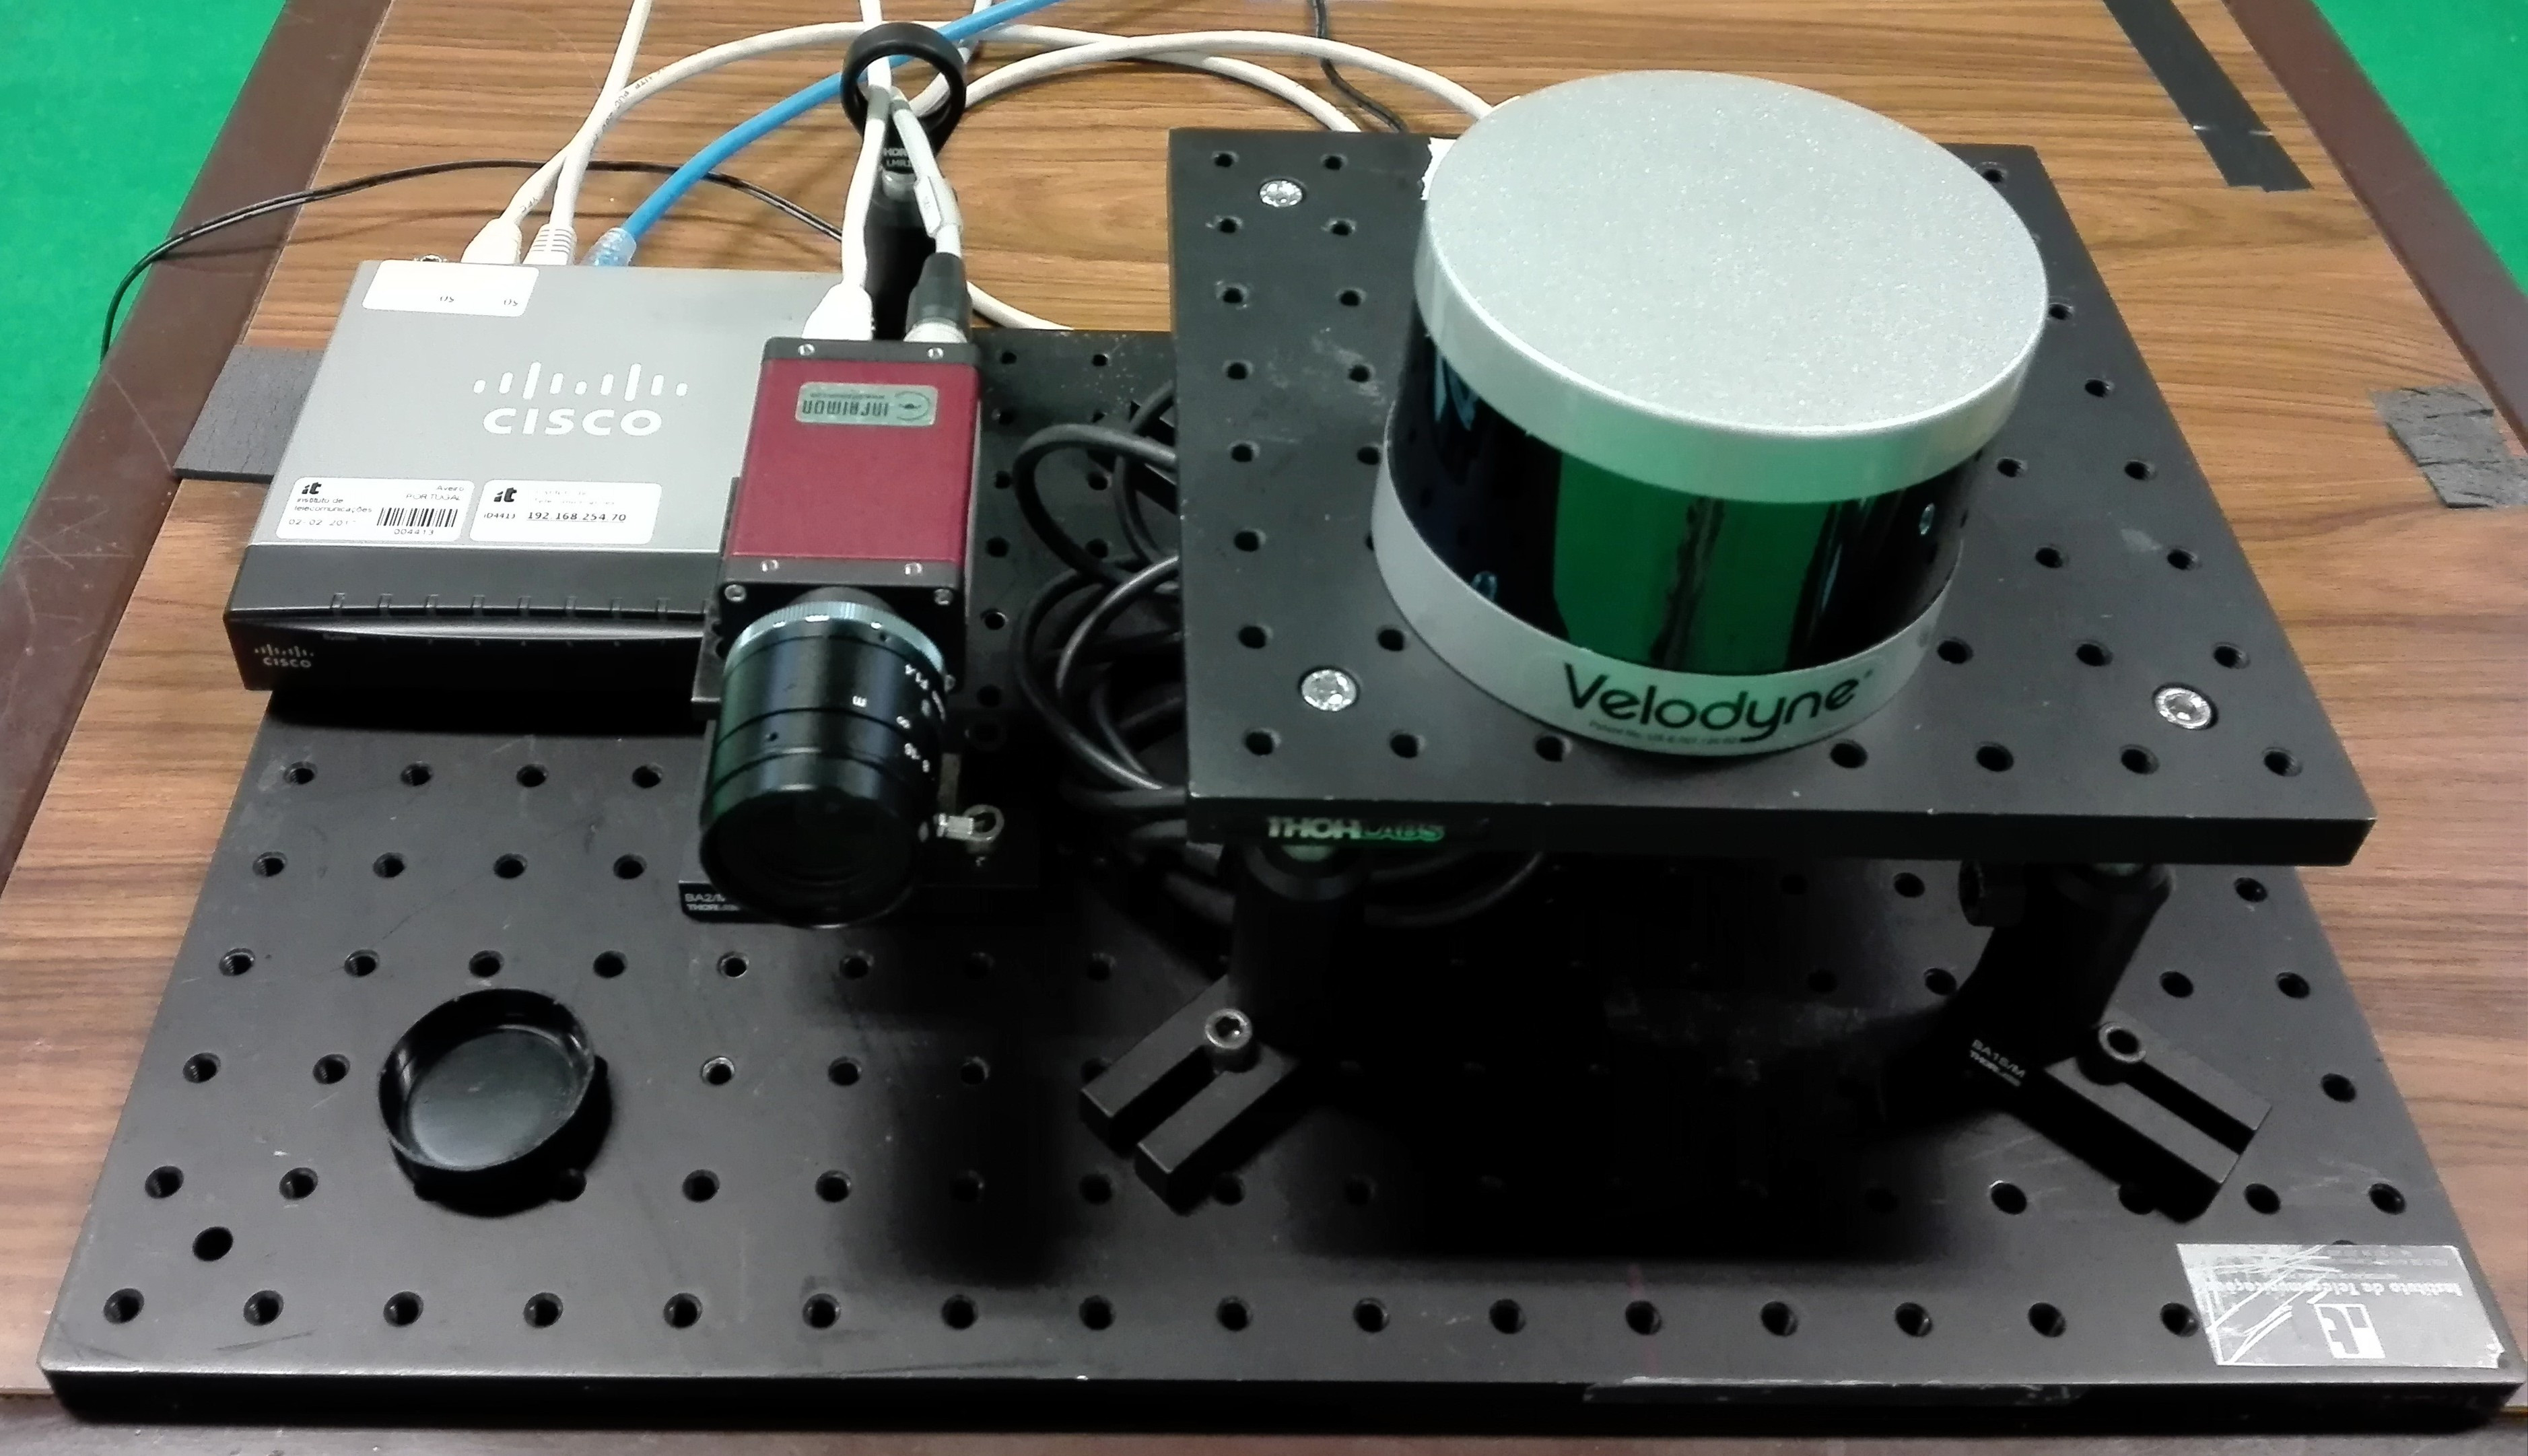
\includegraphics[width=\textwidth]{img/experimental-setup/table-setup-cambada-perspective.jpg}
		\caption{Experimental Setup viewed in perspective.}
		\label{fig:experimental-setup:perspective}
	\end{subfigure}
	\qquad
	\begin{subfigure}[c]{0.45\textwidth}
		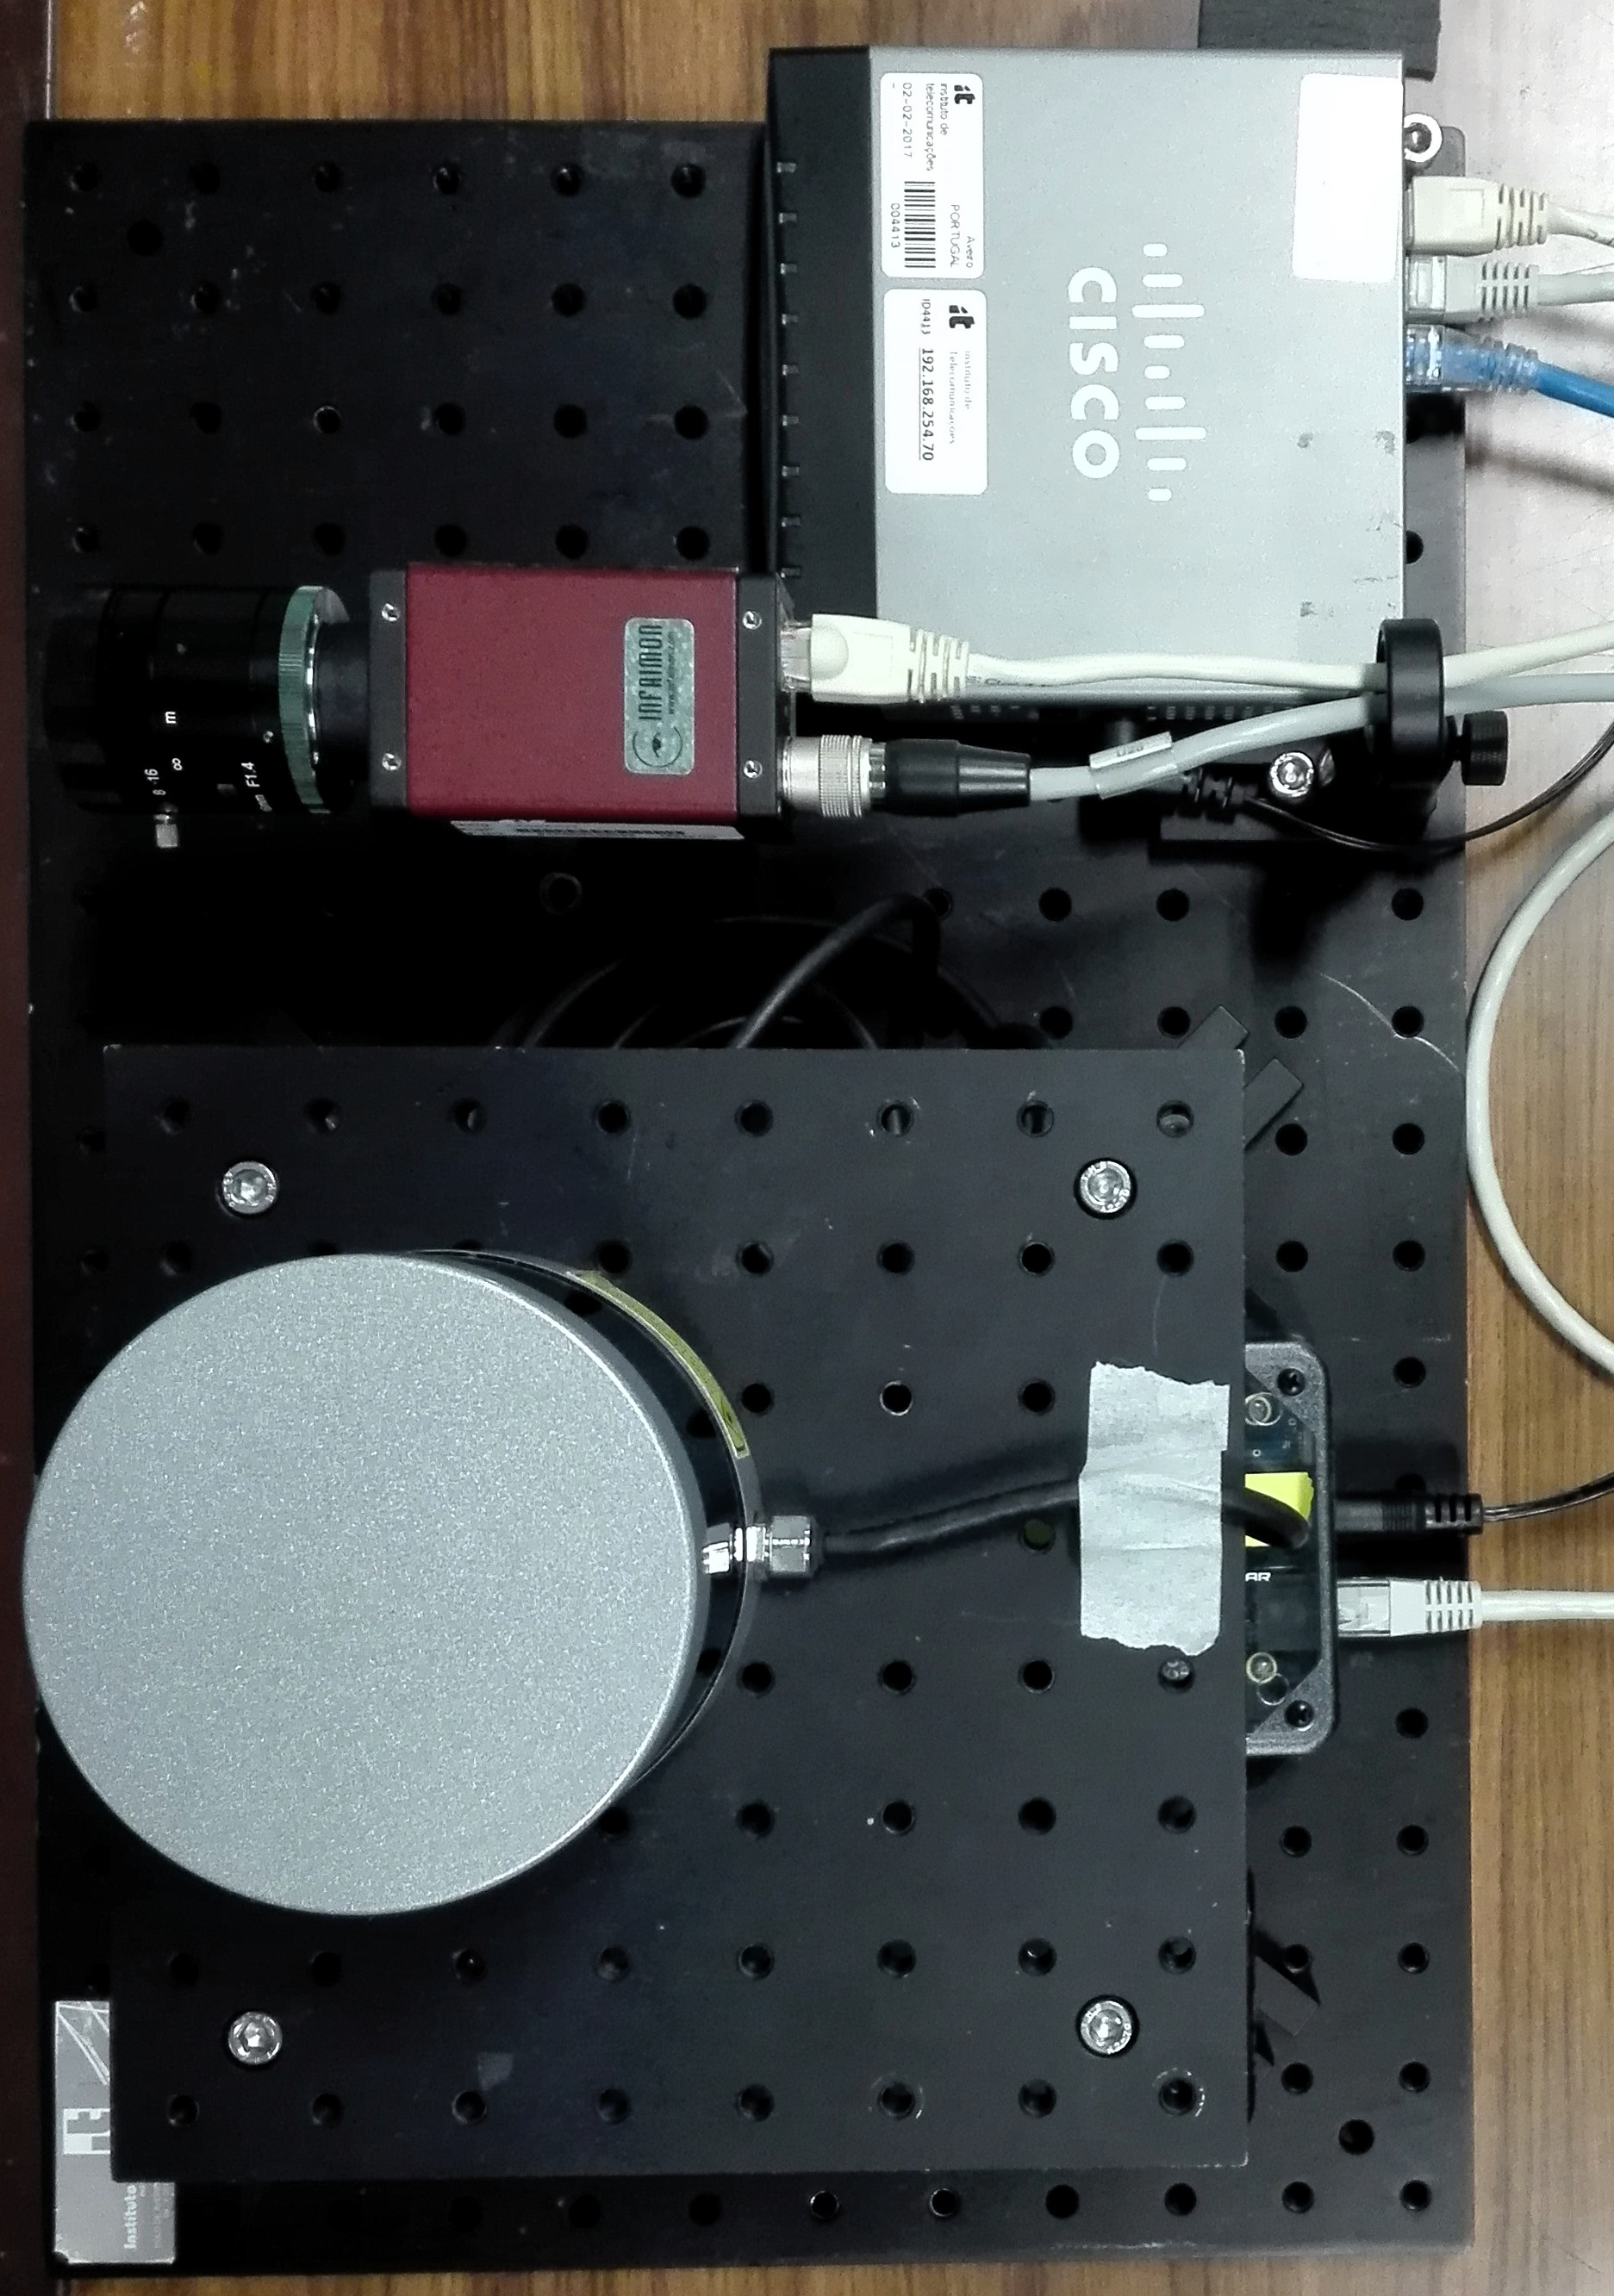
\includegraphics[width=0.65\textwidth, keepaspectratio, angle=90]{img/experimental-setup/table-setup-cambada-birds-eye.jpg}
		\caption{Experimental Setup viewed from the top.}
		\label{fig:experimental-setup:birds-eye}
	\end{subfigure}
	\caption{Relative positioning of the devices on the experimental. The \ac{lidar} is on an elevated platform to guarantee that the camera and Ethernet switch are not on its \ac{fov}.}
	\label{fig:experimental-setup}
\end{figure}

\subsection{Camera and Lens}
The camera used is an industrial 5 \ac{mp} RGB camera, from \acf{avt}  Manta G-504C. Camera lens is a 1" C-Mount format camera with lock from Thorlabs\cp, MVL16M1. The full camera specifications can be accessed on~\cite{MantaG504C} and the full lens specifications on~\cite{Thorlabs}. Relevant specifications of the camera and lens are summarized  on table~\ref{tab:camera-and-lens-specs}. 

\begin{table}[H]
	\renewcommand{\arraystretch}{1.2}
	\centering
	\begin{tabular}{@{}lp{7cm}l@{}}
		\toprule
		\multicolumn{2}{l}{Specification} & Value \\ \midrule
		\multicolumn{2}{l}{\emph{Camera}} & \\
		\phantom{a} & Full Resolution (width vs height) & $2452 \times 2056$   \\
									& Shutter mode & Global \\
									&	Maximum \ac{fps} at full resolution & $9.2$ \\ \midrule 
									\multicolumn{2}{l}{\emph{Lens}} \\
									&	Focal Length & $16$ mm \\
									&	Max aperture & $f/1.4$ \\
									&	Minimum Object Distance & $300$ mm  \\
									& \acs{adc}\footnotemark bit depth & $12$ bit \\
		\bottomrule
	\end{tabular}
	\caption{Relevant specifications for \ac{avt} Manta G-504C RGB camera (from~\cite{MantaG504C})  and MVL16M1 Thorlabs\cp~lens (from~\cite{Thorlabs}).}
	\label{tab:camera-and-lens-specs}
\end{table}

\footnotetext{\acs{adc} stands for \acl{adc}}

To power the Manta G-504C, a laboratory power source must be used. Manta consumes $3.9 W$~\cite{MantaG504C} while operating, accepting an input voltage between $8$ and $30$ $V_{DC}$. The power source used was set to  $12 V_{DC}$ and the current output was $\approx 0.33A$. Voltage and current were measured during all tests, and summarized qualitative results are presented on table~\ref{tab:manta-power}. The power cable provided is a U20 \ac{udp} cable with a HIROSE HR10A-10P-12S female connector. Since the mapping from the 8 pins \ac{udp} cable to the 12 pin connector was not available, a continuity test was made between the expected pinout of the power cable (for more details, see~\cite{AVTCables}) and its the real pinout. The results can be consulted in~\nameref{sec:appendix-b}, on table~\ref{tab:manta-power-cable-pinout}.

	
\begin{table}[H]
	\centering
	\renewcommand{\arraystretch}{1.2}
	\renewcommand{\tabcolsep}{0.45cm}
	\begin{tabular}{@{}llll@{}}
		\toprule
					  & Minimum & Maximum & Median Value \\ \midrule
		Current ($mA$) & $298 \pm 1$ & $330\pm 1$ & $312 \pm 1$ \\
		Voltage ($V$)  & $12.00\pm 0.07 $ & $12.18\pm 0.07$ & $12.08\pm0.07$ \\
		\bottomrule
	\end{tabular}
	\centering
	\caption{Voltage and Current measurements during Manta AVT G-504C operation. Minimum and Maximum values were registered, along with the median. The voltage errors were measured with an Univolt DT-64 multimeter and the current errors were measured on the power source digital display.}
	\label{tab:manta-power}
\end{table}



\subsection{\ac{tof} \ac{lidar}}
The \ac{tof} \ac{lidar} used is a Velodyne VLP-16\texttrademark, a 16 beam \ac{lidar} that operates with a wavelength of $903 nm$. VLP-16 supports various measurements modes based on the return pulse (Strongest, Last, Dual) and can be connected to a \ac{gps} receiver for geopositioning and synchronization with an external clock. It also supports several rotation velocities, from 300 to 1200 \ac{rpm}, which result in different angular steps and point cloud refresh rate. The full specifications can be accessed on~\cite{VLP16} and the relevant specifications for this work are summarized on table~\ref{tab:vlp16-specs}.

\begin{table}[H]
	\renewcommand{\arraystretch}{1.2}
	\centering
	\begin{tabular}{@{}p{8.3cm}l@{}}
		\toprule
		Specification & Value \\ \midrule
		Wavelength    & 903 nm \\
		Motor \acs{rpm} & $600 \pm 3$ \\
		Angular step & 0.2º \\
		Vertical \ac{fov} & 30º \\
		Horizontal \ac{fov} & 360º \\
		Maximum Scanning Distance & 100m \\
		Theoretical Maximum Distance Error & $2 cm$ \\
		\bottomrule
	\end{tabular}
	\caption{Velodyne VLP-16 relevant specifications. Source~\cite{VLP16}.}
	\label{tab:vlp16-specs}
\end{table}


\subsection{Setup Connection} 
Both Velodyne VLP-16 and \ac{avt} Manta G-504C operate over Gigabit Ethernet. Therefore, a Gigabit  Ethernet switch is required to connect all the equipment to a single computer using a single Ethernet port. The switch used was Cisco SG200-08, an 8-Port Gigabit Smart Switch. 

The switch was configured so that every port was on the same \ac{vlan}, ensuring packets were accessible on the computer, since the sensors were configured to broadcast the packets. An alternative to this implementation was to redirect the packets from each sensor to the computer network and filter the packets from the computer to the sensors, by putting them on separated networks and create a network traffic management solution. However, since no bandwidth constraints or packet delay/loss were verified, the solution chosen was the former, due to its simplicity. 

For each device a fixed \acf{ip} address as attributed, following the instructions on their datasheet~\cite{VLP16, MantaVision2013}. The \acp{ip} addresses can be consulted on table~\ref{tab:experimental-setup-ip}.

\begin{table}[H]
	\renewcommand{\arraystretch}{1.2}
	\centering
	\begin{tabular}{@{}lcc@{}}
		\toprule
		Device          & \ac{ip} Address & Subnet Mask\\ \midrule
		Computer        & 192.168.10.77  & 255.255.255.0 \\
		Manta G-504C    & 192.168.10.1   & 255.255.255.0 \\
		Velodyne VLP-16 & 192.168.10.201 & 255.255.255.0 \\
		\bottomrule
	\end{tabular}
	\caption{\acp{ip} and subnet masks for the devices connected on the experimental setup.}
	\label{tab:experimental-setup-ip}
\end{table}

\subsection{\ac{lidar} and Camera Interference}
No significant interference is expected between the camera and the \ac{lidar}. Despite the camera lens having a transmission coefficient of $66\%$ at $\approx 900 nm$~\cite{Thorlabs}, Sony ICX655, the camera sensor for the \ac{avt} Manta G-504C, only was a Quantum Efficiency of $\approx 5\%$~\cite{MantaG504C}. \ac{avt} Manta G-504C can also be equipped with an \ac{ir} cut-filter, that can be selected on purchase. However, such information was not available.

Despite the low sensibility of the camera and the possibility of an \ac{ir} cut-filter being present, an experiment was conducted to verify the occurrence of interference. The experimental setup was switched on in a Dark Room without any light sources switched on and the camera feed was visualized. Besides the noise caused by the camera electronics operation, no signs of interference caused by the \ac{lidar} infrared beams could be seen on the camera image feed. Therefore, no further research on \ac{lidar} to camera interference were carried


%\begin{figure}[H]
%	\centering
%	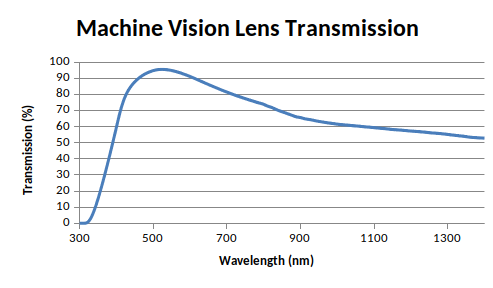
\includegraphics[width=0.6\textwidth]{img/experimental-setup/lens-transmission.png}
%	\caption{Transmission of the MVL16M1 lens in relation the light wavelength. Source~\cite{Thorlabs}}
%	\label{fig:lens-transmission}
%\end{figure}



\section{Camera Intrinsic Calibration}
\label{sec:calibration:camera}
The act of calibrating a camera consists on determining its intrinsic parameters, as detailed in subsection~\ref{subsec:sota:camera-intrinisc-calibration}. This can be done by taking different images with a known pattern, fully visible on the camera \ac{fov}, changing its rotation and translation in relation to the camera coordinate frame.

The calibration procedure undertaken uses a chessboard of $13 \times 9$ squares, with each square having an edge length of $44.0 mm$. The chessboard used can be seen on figure~\ref{fig:chessboard}. It was laser printed on a 100gr A2 paper and then glued to a plywood board.

\begin{figure}[H]
	\centering
	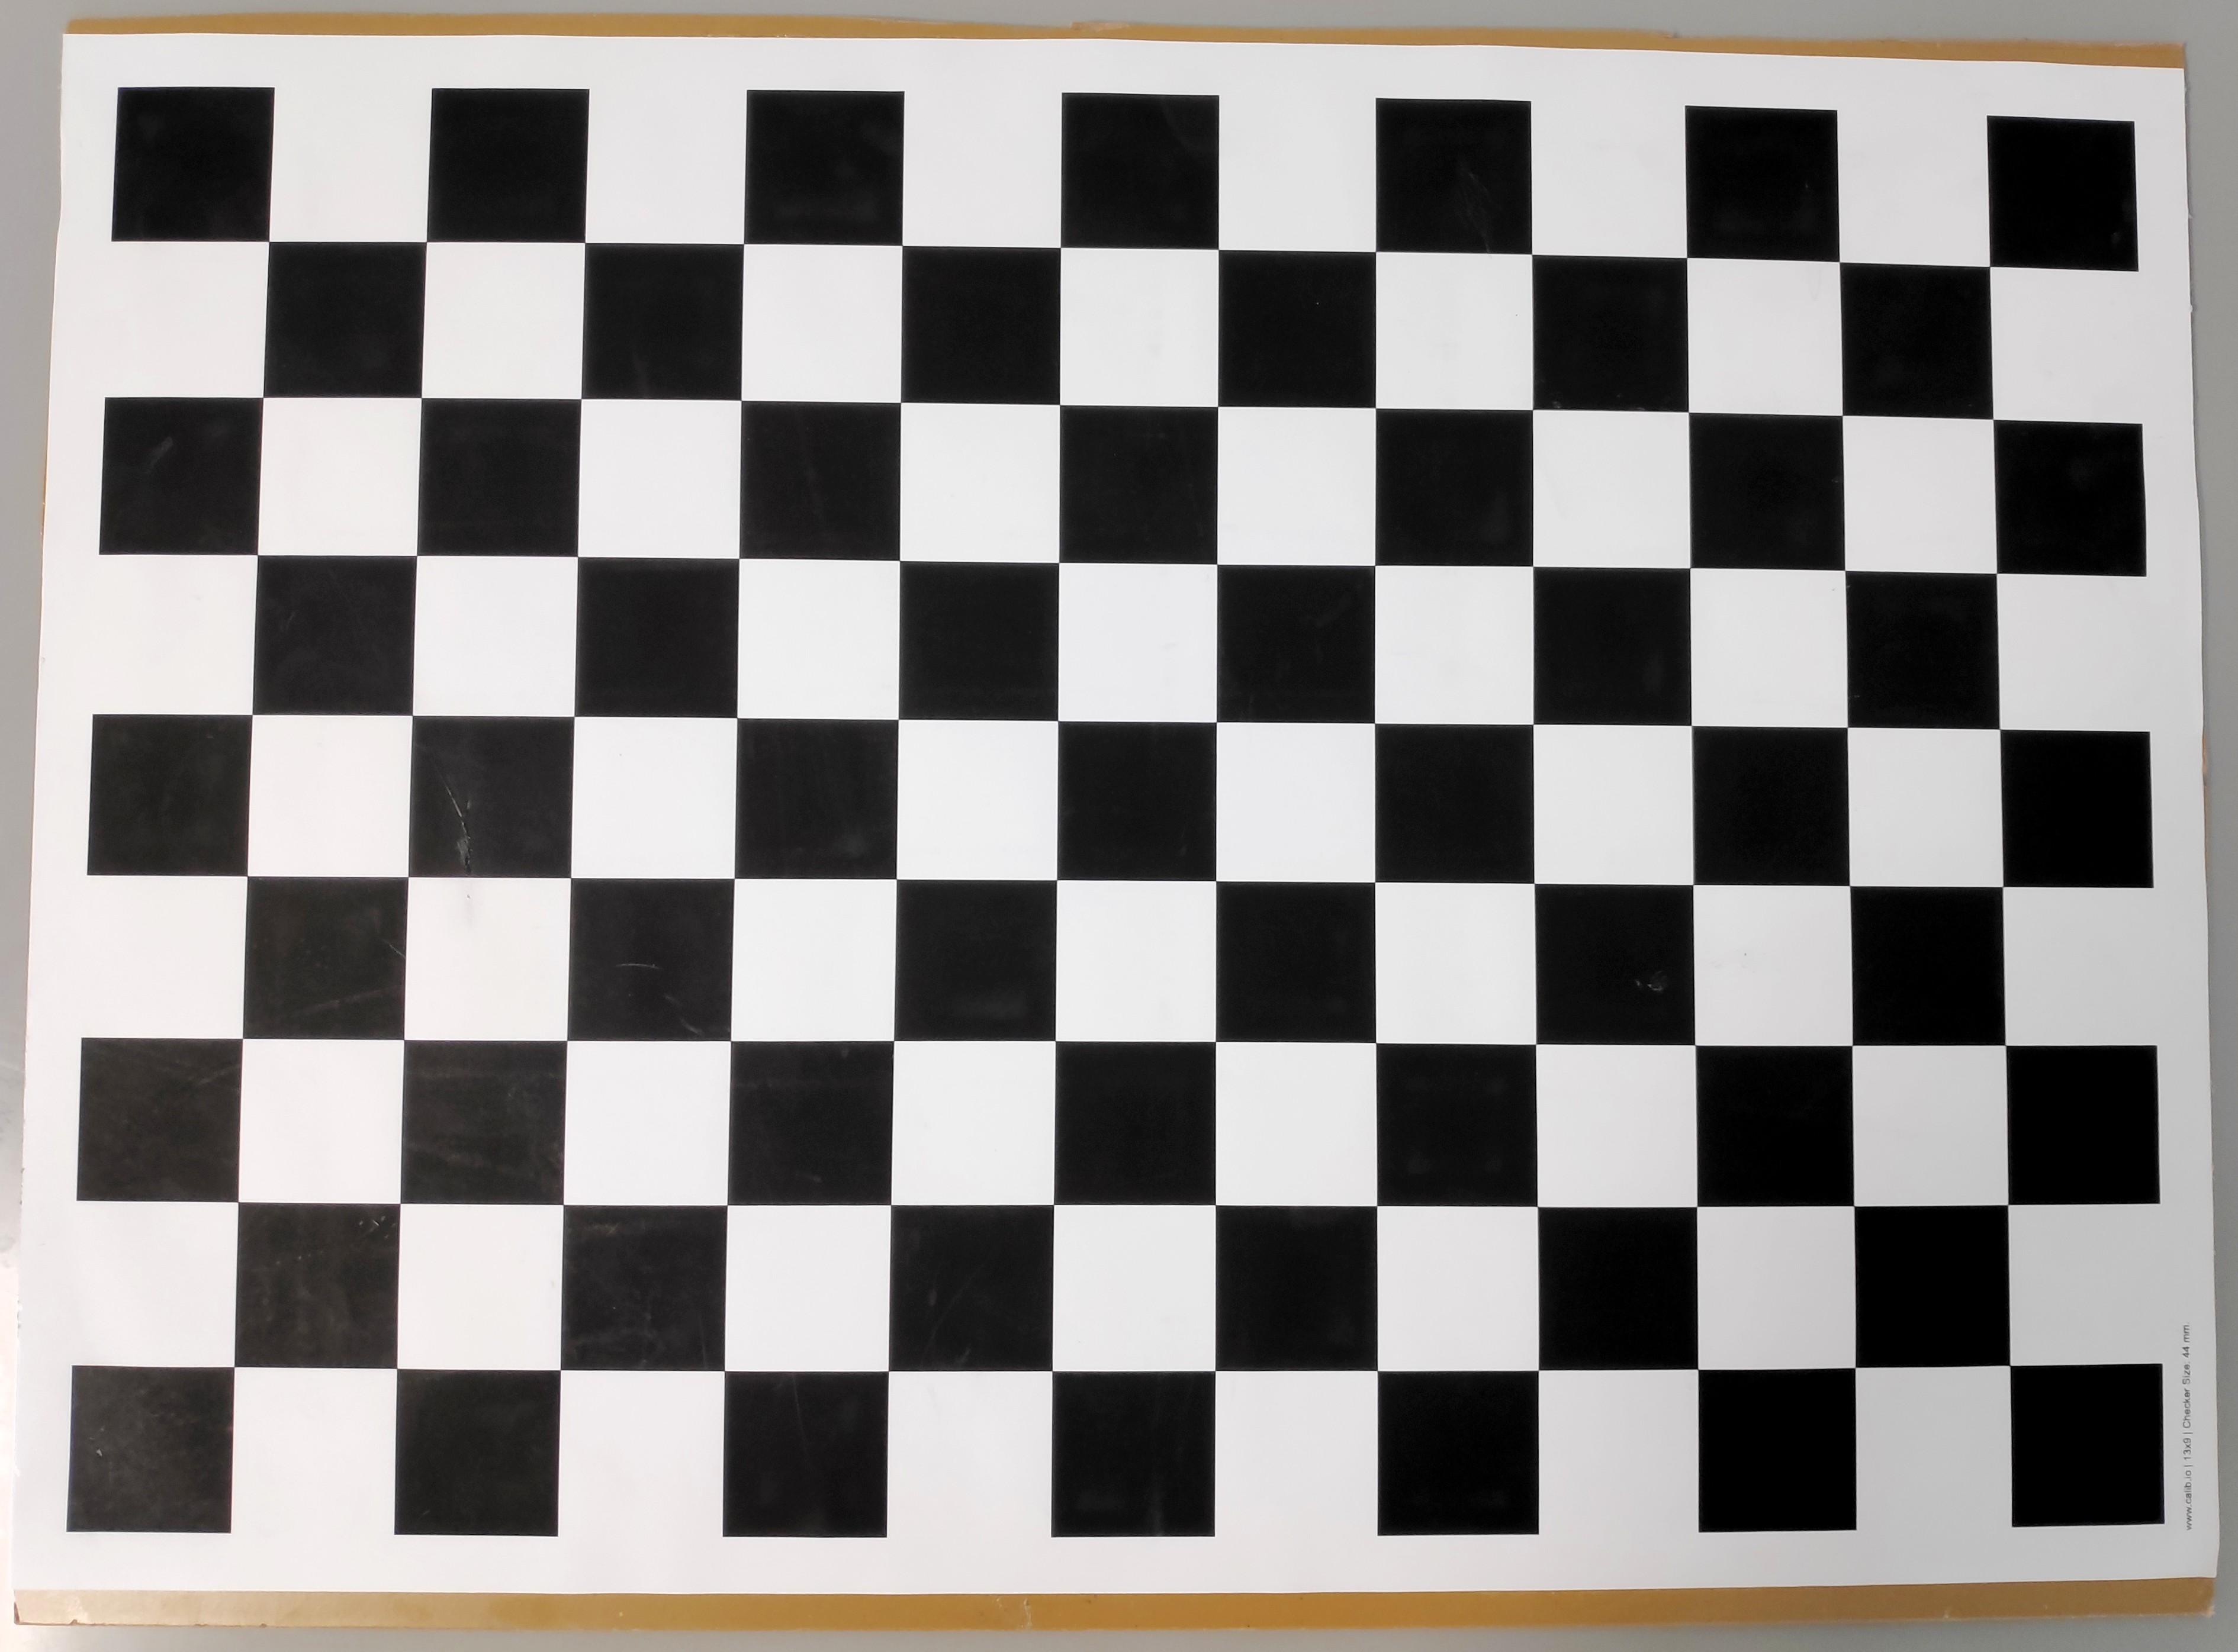
\includegraphics[width=0.5\textwidth]{img/experimental-setup/chessboard.jpg}
	\caption{Chessboard used during camera calibration procedures. The chessboard was laser printed on A2 paper size, in real size, that was then glued to a plywood board.}
	\label{fig:chessboard}
\end{figure}

Calibrating the camera requires that the calibration object to be focused. Therefore, before any proper calibration can be made, focus theory and procedure are given on the next sub-section,~\ref{subsec:calibration:camera-focus}.


\subsection{Camera Focus and \acl{dof}}
\label{subsec:calibration:camera-focus}
Focusing a camera can only be attained for an exact distance from the camera~\cite{Merklinger1993, Photopillers}, measured perpendicularly to the plane of focus, which is the plane containing the \ac{cmos} or \ac{ccd} chip. Therefore, on every image, there is a plane of focus and what actually ``looks focused'' is really just in ``acceptably sharp focus'', since precise focus is only possible to an exact distance, and not for an entire tridimensional object.

``Acceptably sharp focus'' means that a point in the real world would not result in a point on the image (as happens in precise focus), but in a blurred spot that is circular (due to the form of the aperture)\cite{Photopillers}. However, if the size of blur is small enough, little to no differences can be perceived and the image is considered to be focused\cite{Photopillers}. The maximum size at which this blur is not noticed by the viewer (given a specific sensor size, dimension of the viewed photo, viewing distance and acuity of the viewer) is called the \ac{coc}\cite{Photopillers, Merklinger1993}.

The first step in focusing an image requires the calculation of the hyperfocal distance, $H$: the distance at which the camera is focused to ensure objects from half of this distance to the infinity are in an ``acceptably sharp focus'' (refer to as just focus, from now on). This distance can be calculated using the equation~\ref{eq:hyperfocal_distance}, below, where $f$ is the focal length, $F_N$ is the F-number and $c$ the \ac{coc} limit. Hyperfocal near limit is defined as $H_{near} = \rfrac{H}{2}$.

\begin{equation}
	\label{eq:hyperfocal_distance}
	H = \frac{f^2}{F_Nc} + f \approx \frac{f^2}{F_Nc} 
\end{equation}

Known the hyperfocal distance, the \acf{dof} can be calculated. \ac{dof} is measured in meters and is obtained by subtracting the farthest and nearest distances at which an object is focused (see equation~\ref{eq:dof}), indicating the distance between this two points\cite{Photopillers, Merklinger1993, mvg_book}. The nearest and farthest points can be calculated using the equations~\ref{eq:dof-near} and~\ref{eq:dof-far}, respectively.

\begin{subequations}
	\label{eq:dof_all}
	\begin{align}
		DoF & = DoF_{far} - DoF_{near} \label{eq:dof} \\
		DoF_{far} & = \frac{H\times d}{H - (d - f)} \label{eq:dof-far} \\
		DoF_{near} & = \frac{H\times d}{H + (d - f)} \label{eq:dof-near} 
	\end{align}
\end{subequations}

Using equations~\ref{eq:dof_all} is possible to select a desired \acl{dof} for an image that guarantees that all the objects of interest are focused. Taking in consideration that smaller apertures (bigger F-numbers) will increase the exposition time\cite{Merklinger1993}, a target distance can be selected with the guarantee that all the objects from the near \ac{dof} point to the far \ac{dof} will be sharp.

Rewriting the equation~\ref{eq:dof-near} to calculate the objects distance, giving the minimum distance at the objects must be focused, one gets the equation~\ref{eq:dof-subject-distance}.

\begin{equation}
	\label{eq:dof-subject-distance}
	d = \frac{(H - f) \cdot DoF_{near}}{H - DoF_{near}}
\end{equation}


\subsection{Camera Calibration Procedure}
For calibration, \ac{opencv} algorithms are used~\cite{opencv_doc}, such as \emph{calibrateCamera}, \emph{solvePnP} and \emph{findChessboardCorners}. These algorithms, the underling code interconnecting them and a \ac{gui} for performing calibration are available in a \ac{ros} package, \emph{camera\_calibration} from the \emph{image\_pipeline} metapackage~\cite{cameraCalibrationRos}, which is used.

For calibration, around 50 unique photos are taken for each setup. These images are converted to greyscale, the chessboard corners are detected and the camera intrinsic parameters are computed by the \emph{camera\_calibration} ROS package. A subset of the calibration images is presented on figure~\ref{fig:camera-calibration-images}.

\begin{figure}[h]
	\centering
	\begin{subfigure}[c]{0.30\textwidth}
		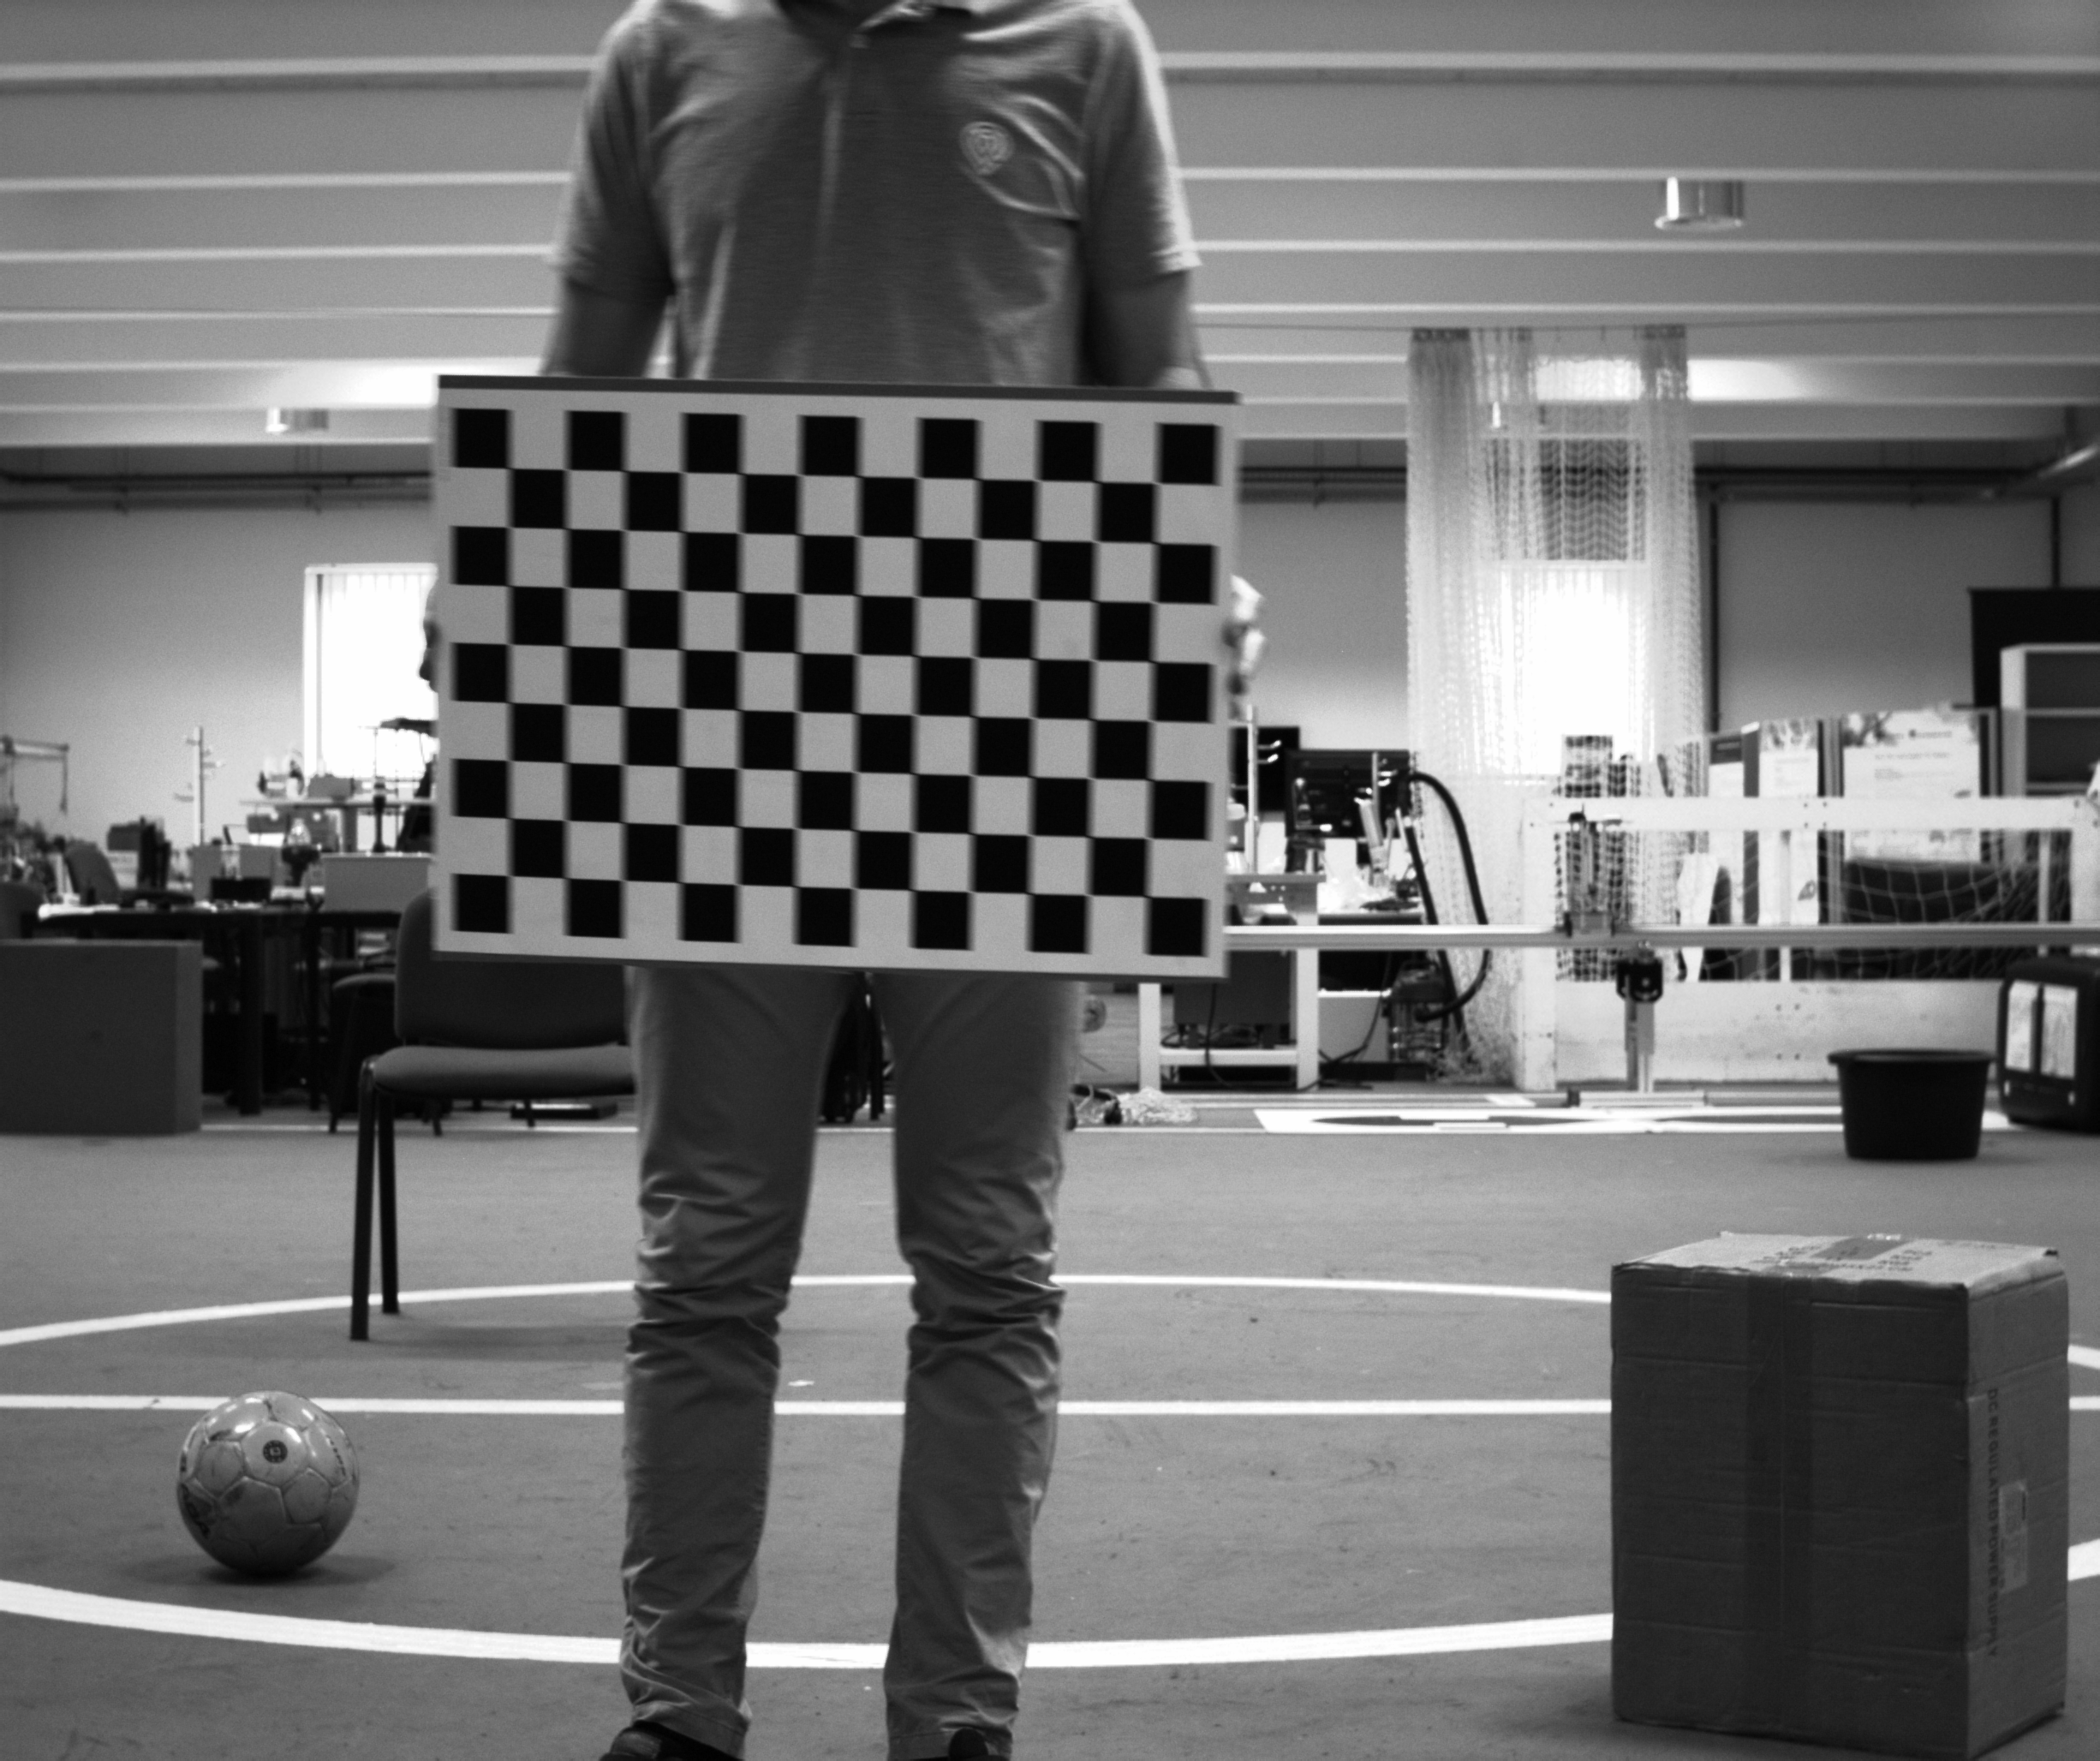
\includegraphics[width=0.9\textwidth]{img/camera-calibration/left-0001.png}
	\end{subfigure}
	\begin{subfigure}[c]{0.30\textwidth}
		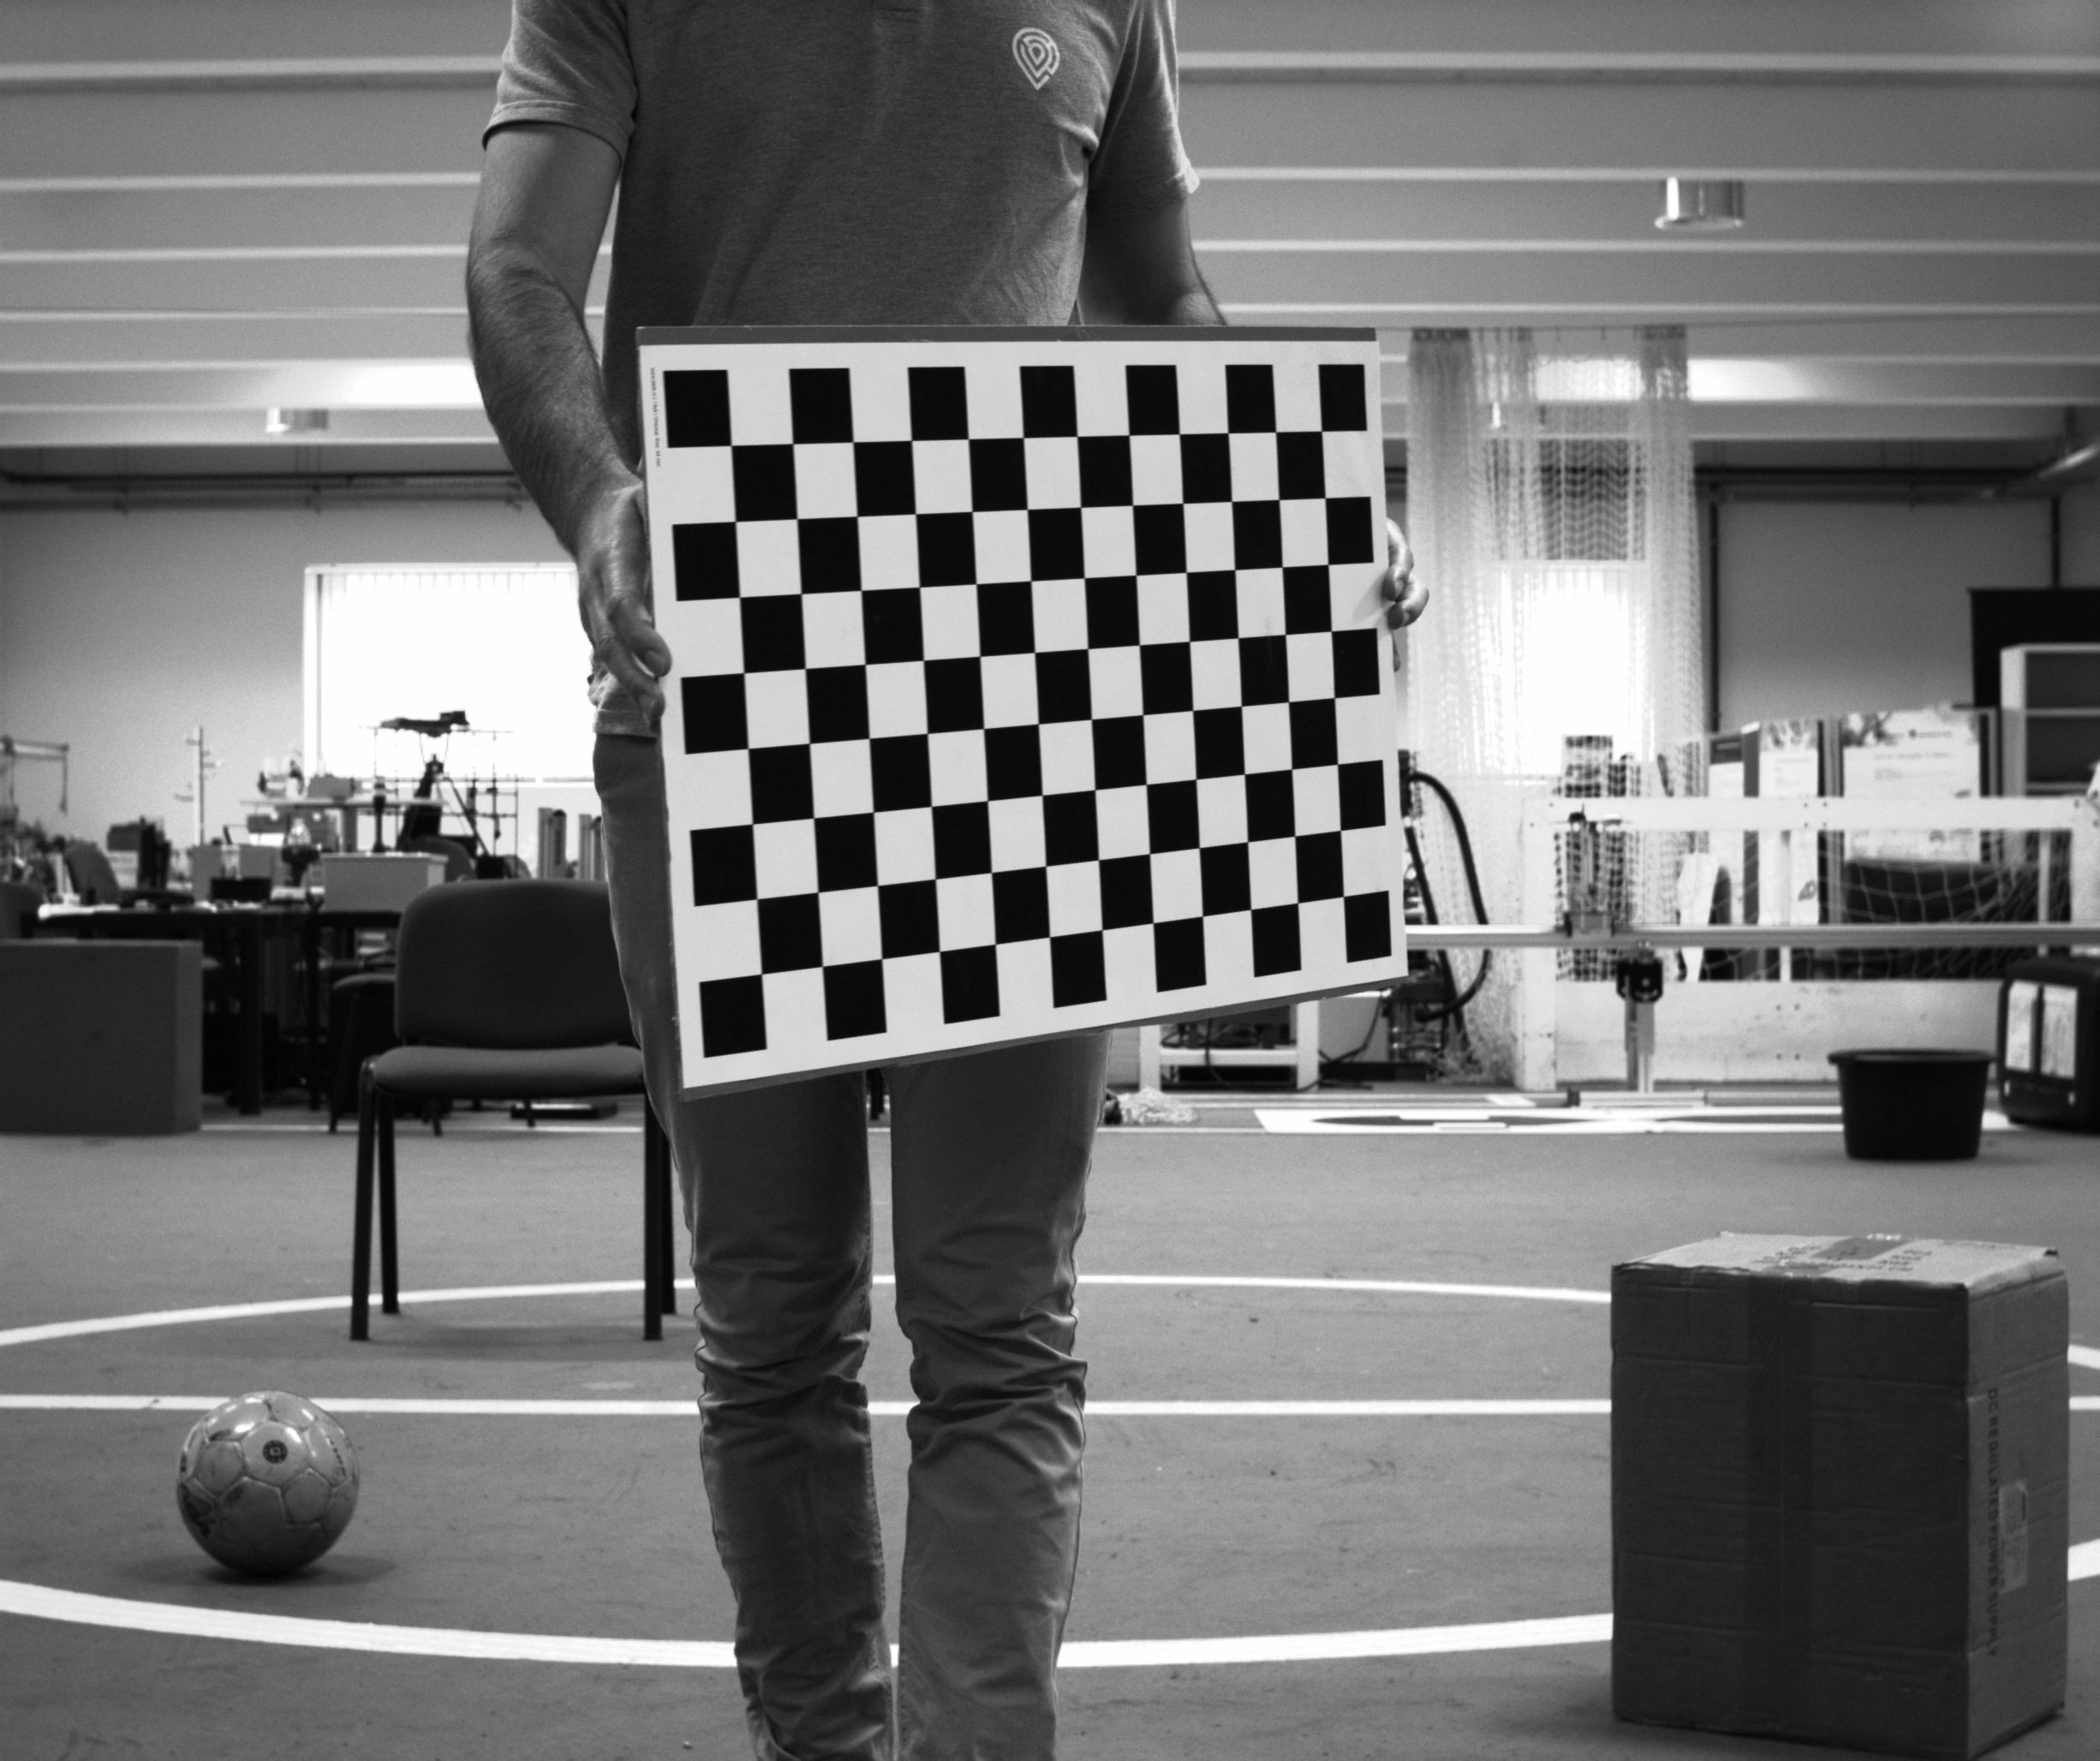
\includegraphics[width=0.9\textwidth]{img/camera-calibration/left-0005.png}
	\end{subfigure}
	\begin{subfigure}[c]{0.30\textwidth}
		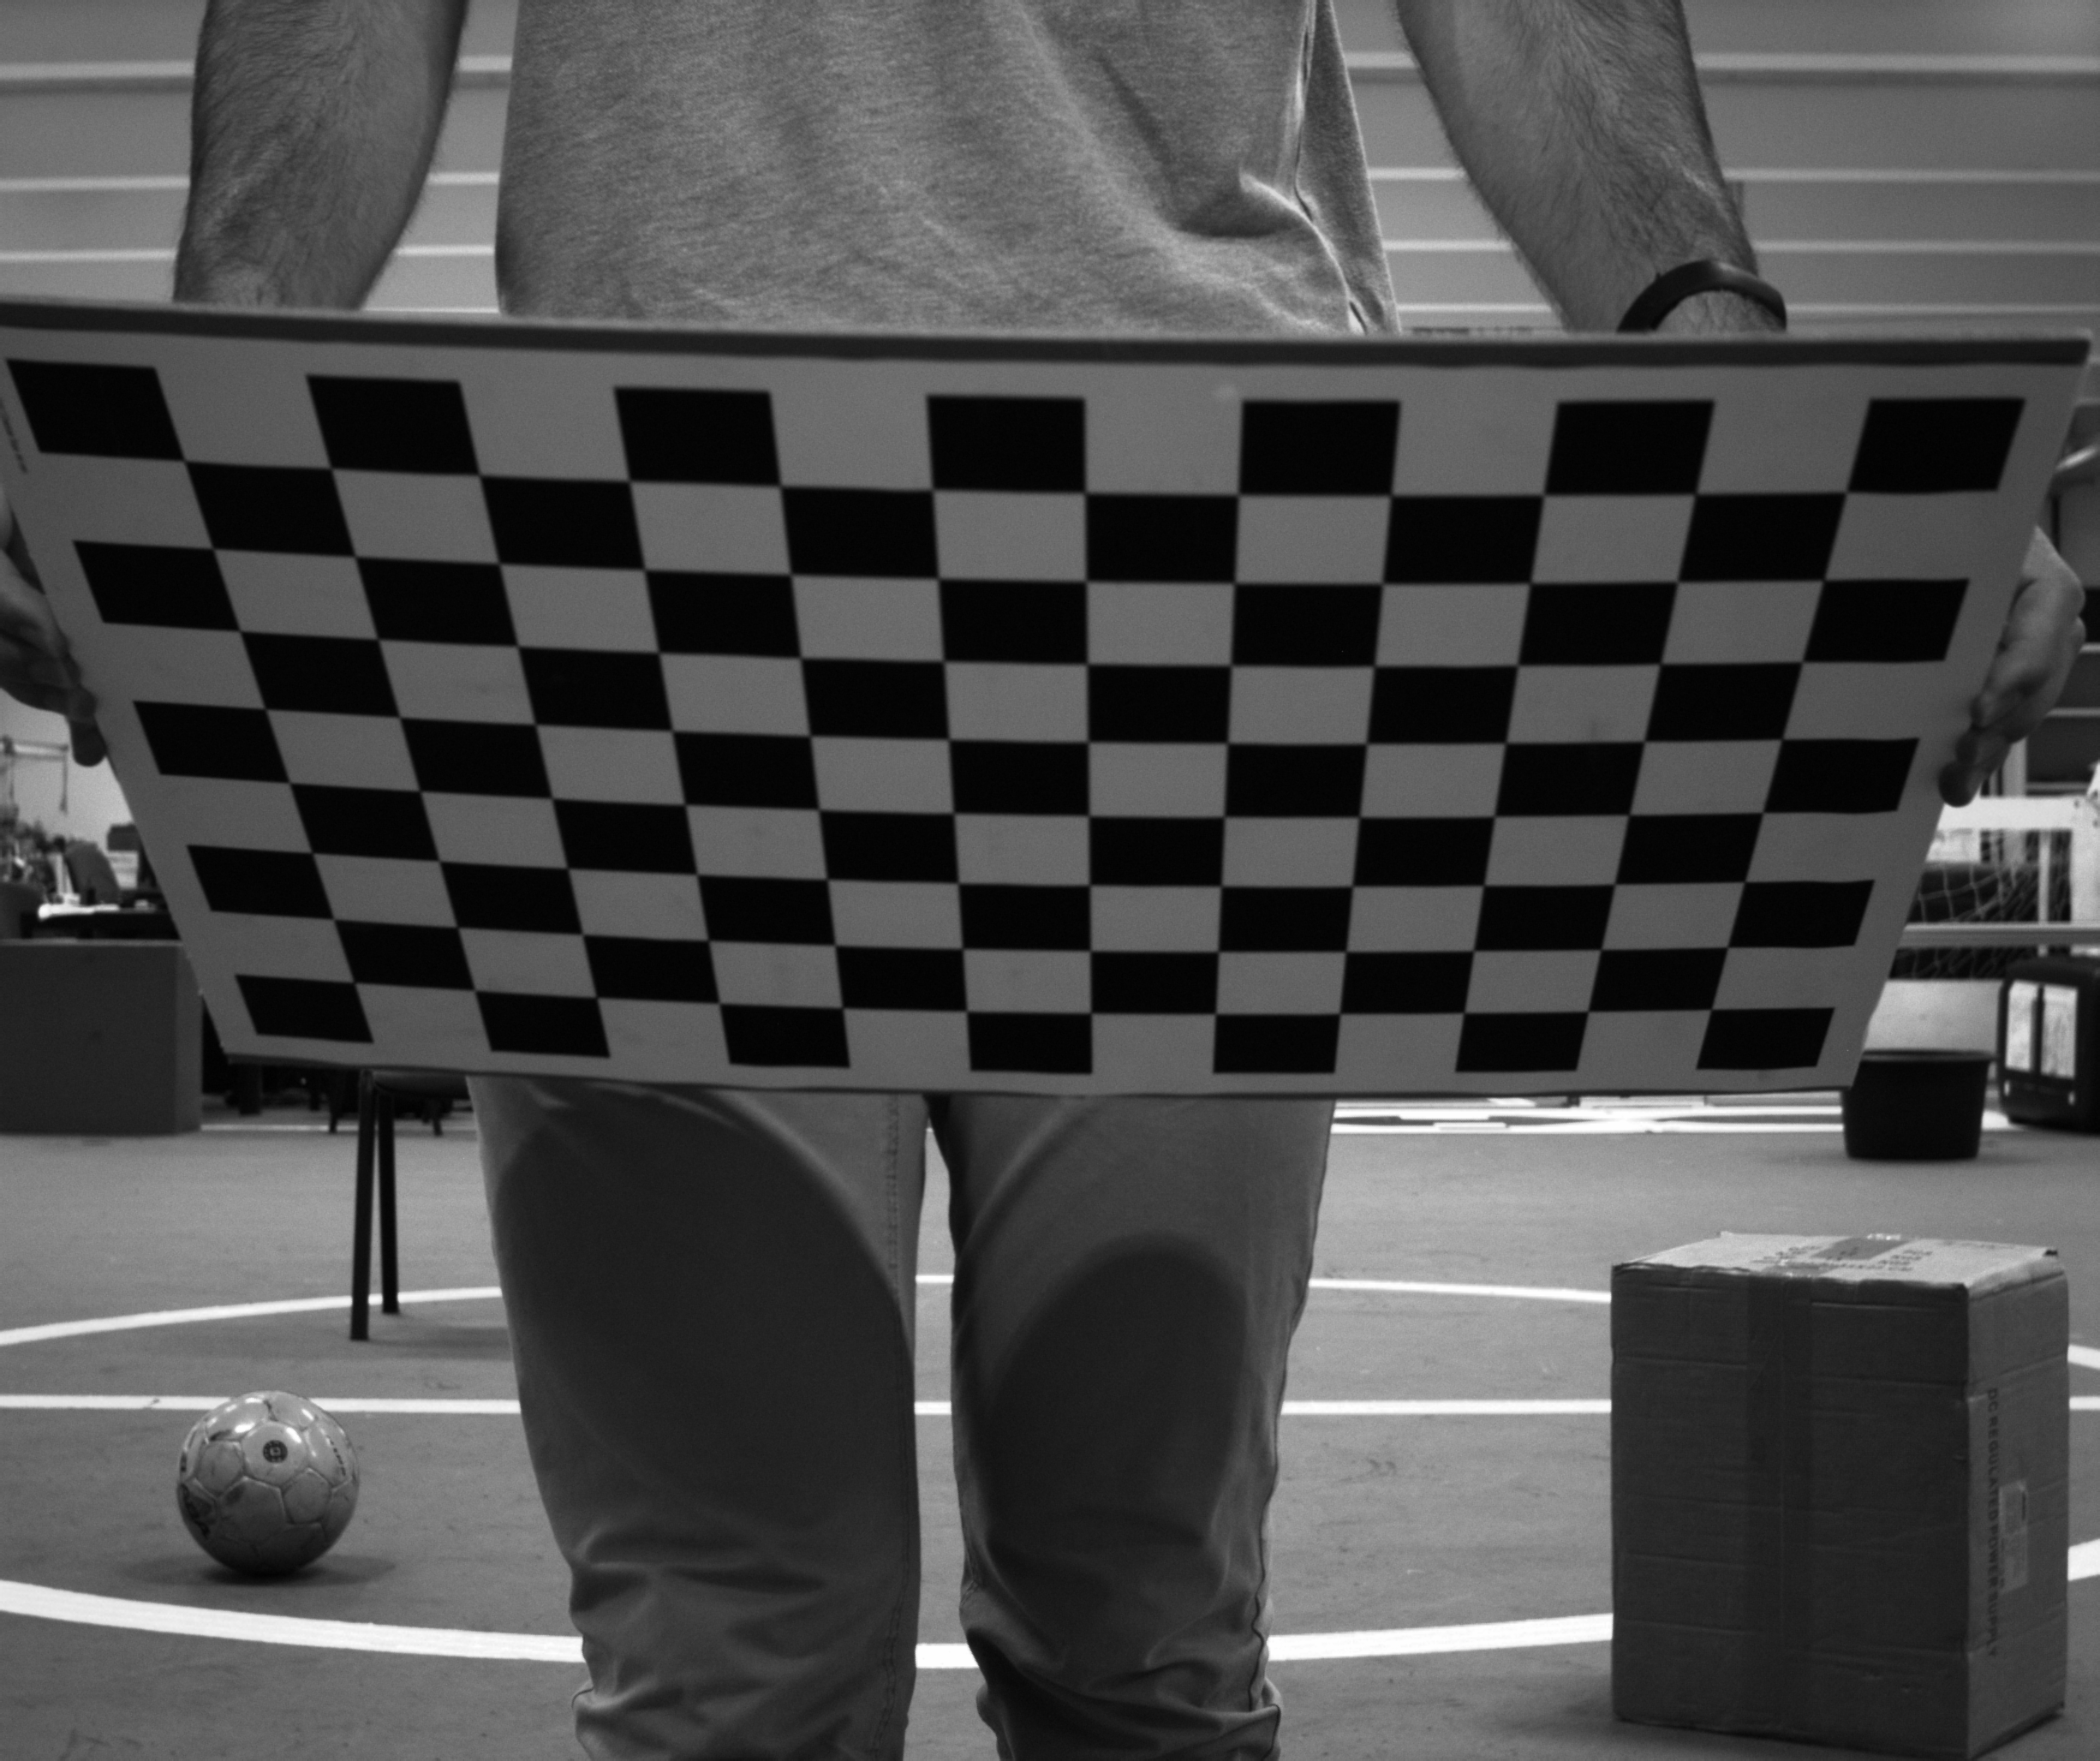
\includegraphics[width=0.9\textwidth]{img/camera-calibration/left-0022.png}
	\end{subfigure}
	\\ 
	\vspace{5mm}
	\begin{subfigure}[c]{0.30\textwidth}
		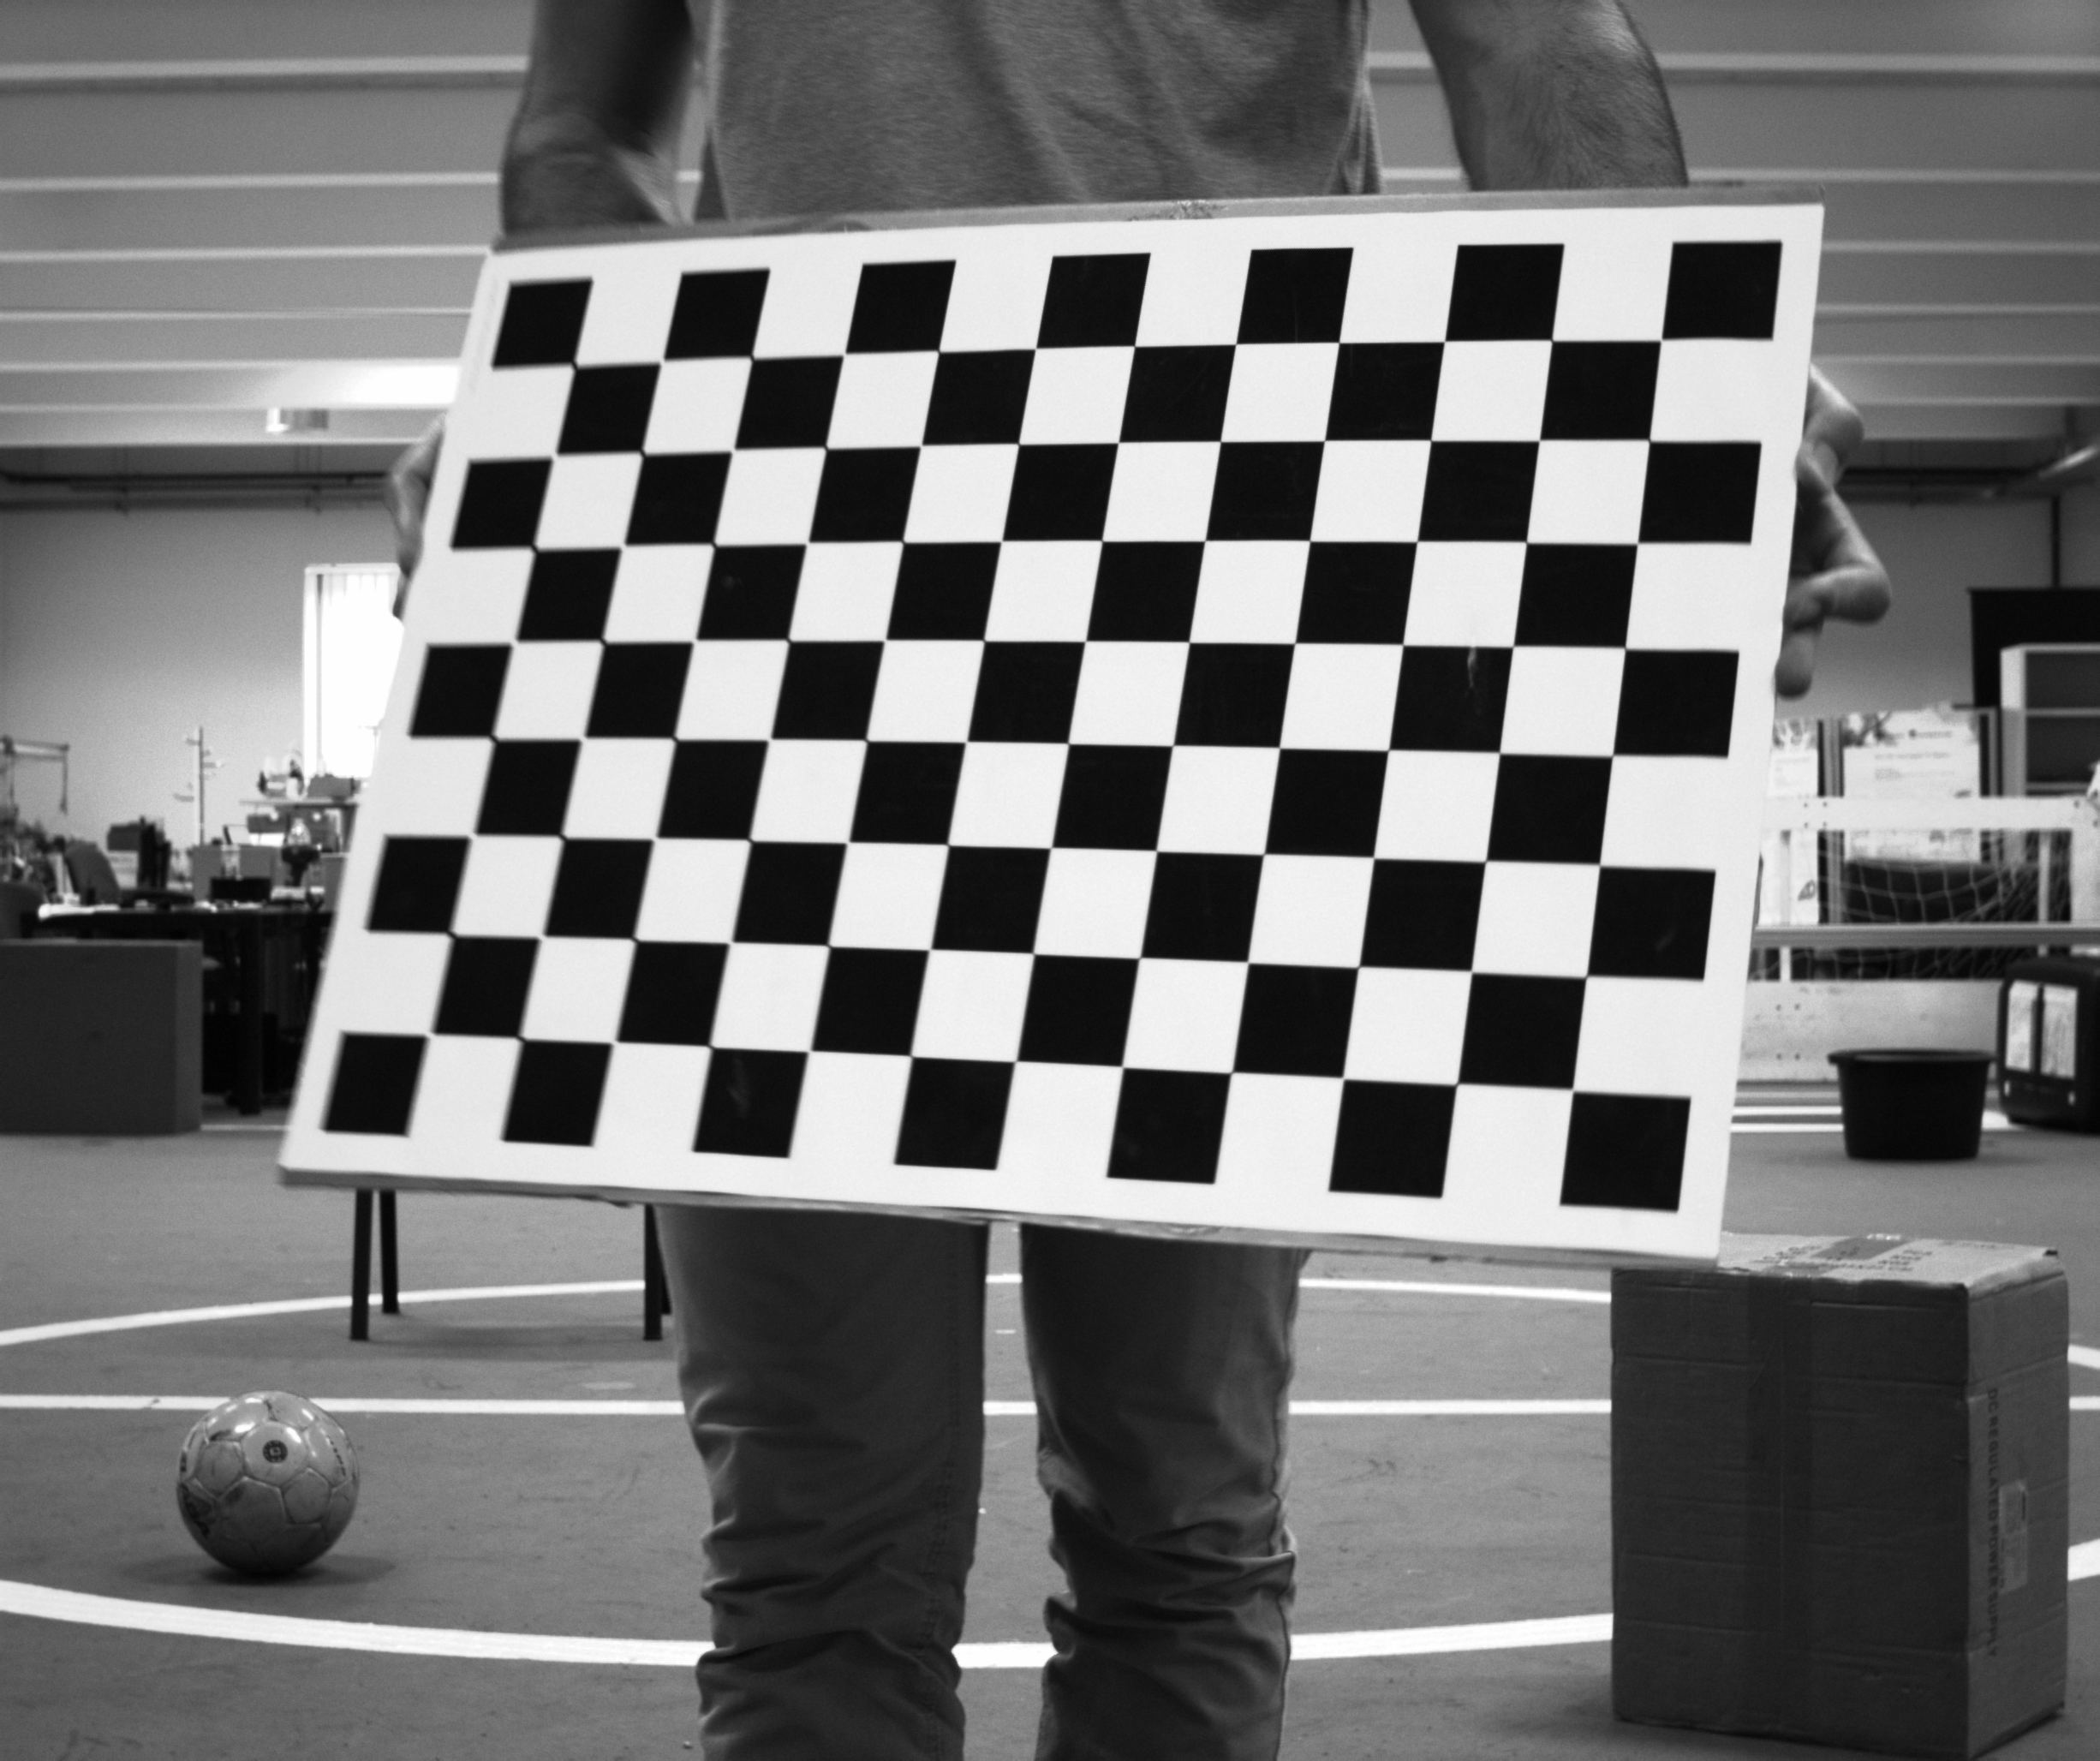
\includegraphics[width=0.9\textwidth]{img/camera-calibration/left-0030.png}
	\end{subfigure}
	\begin{subfigure}[c]{0.30\textwidth}
		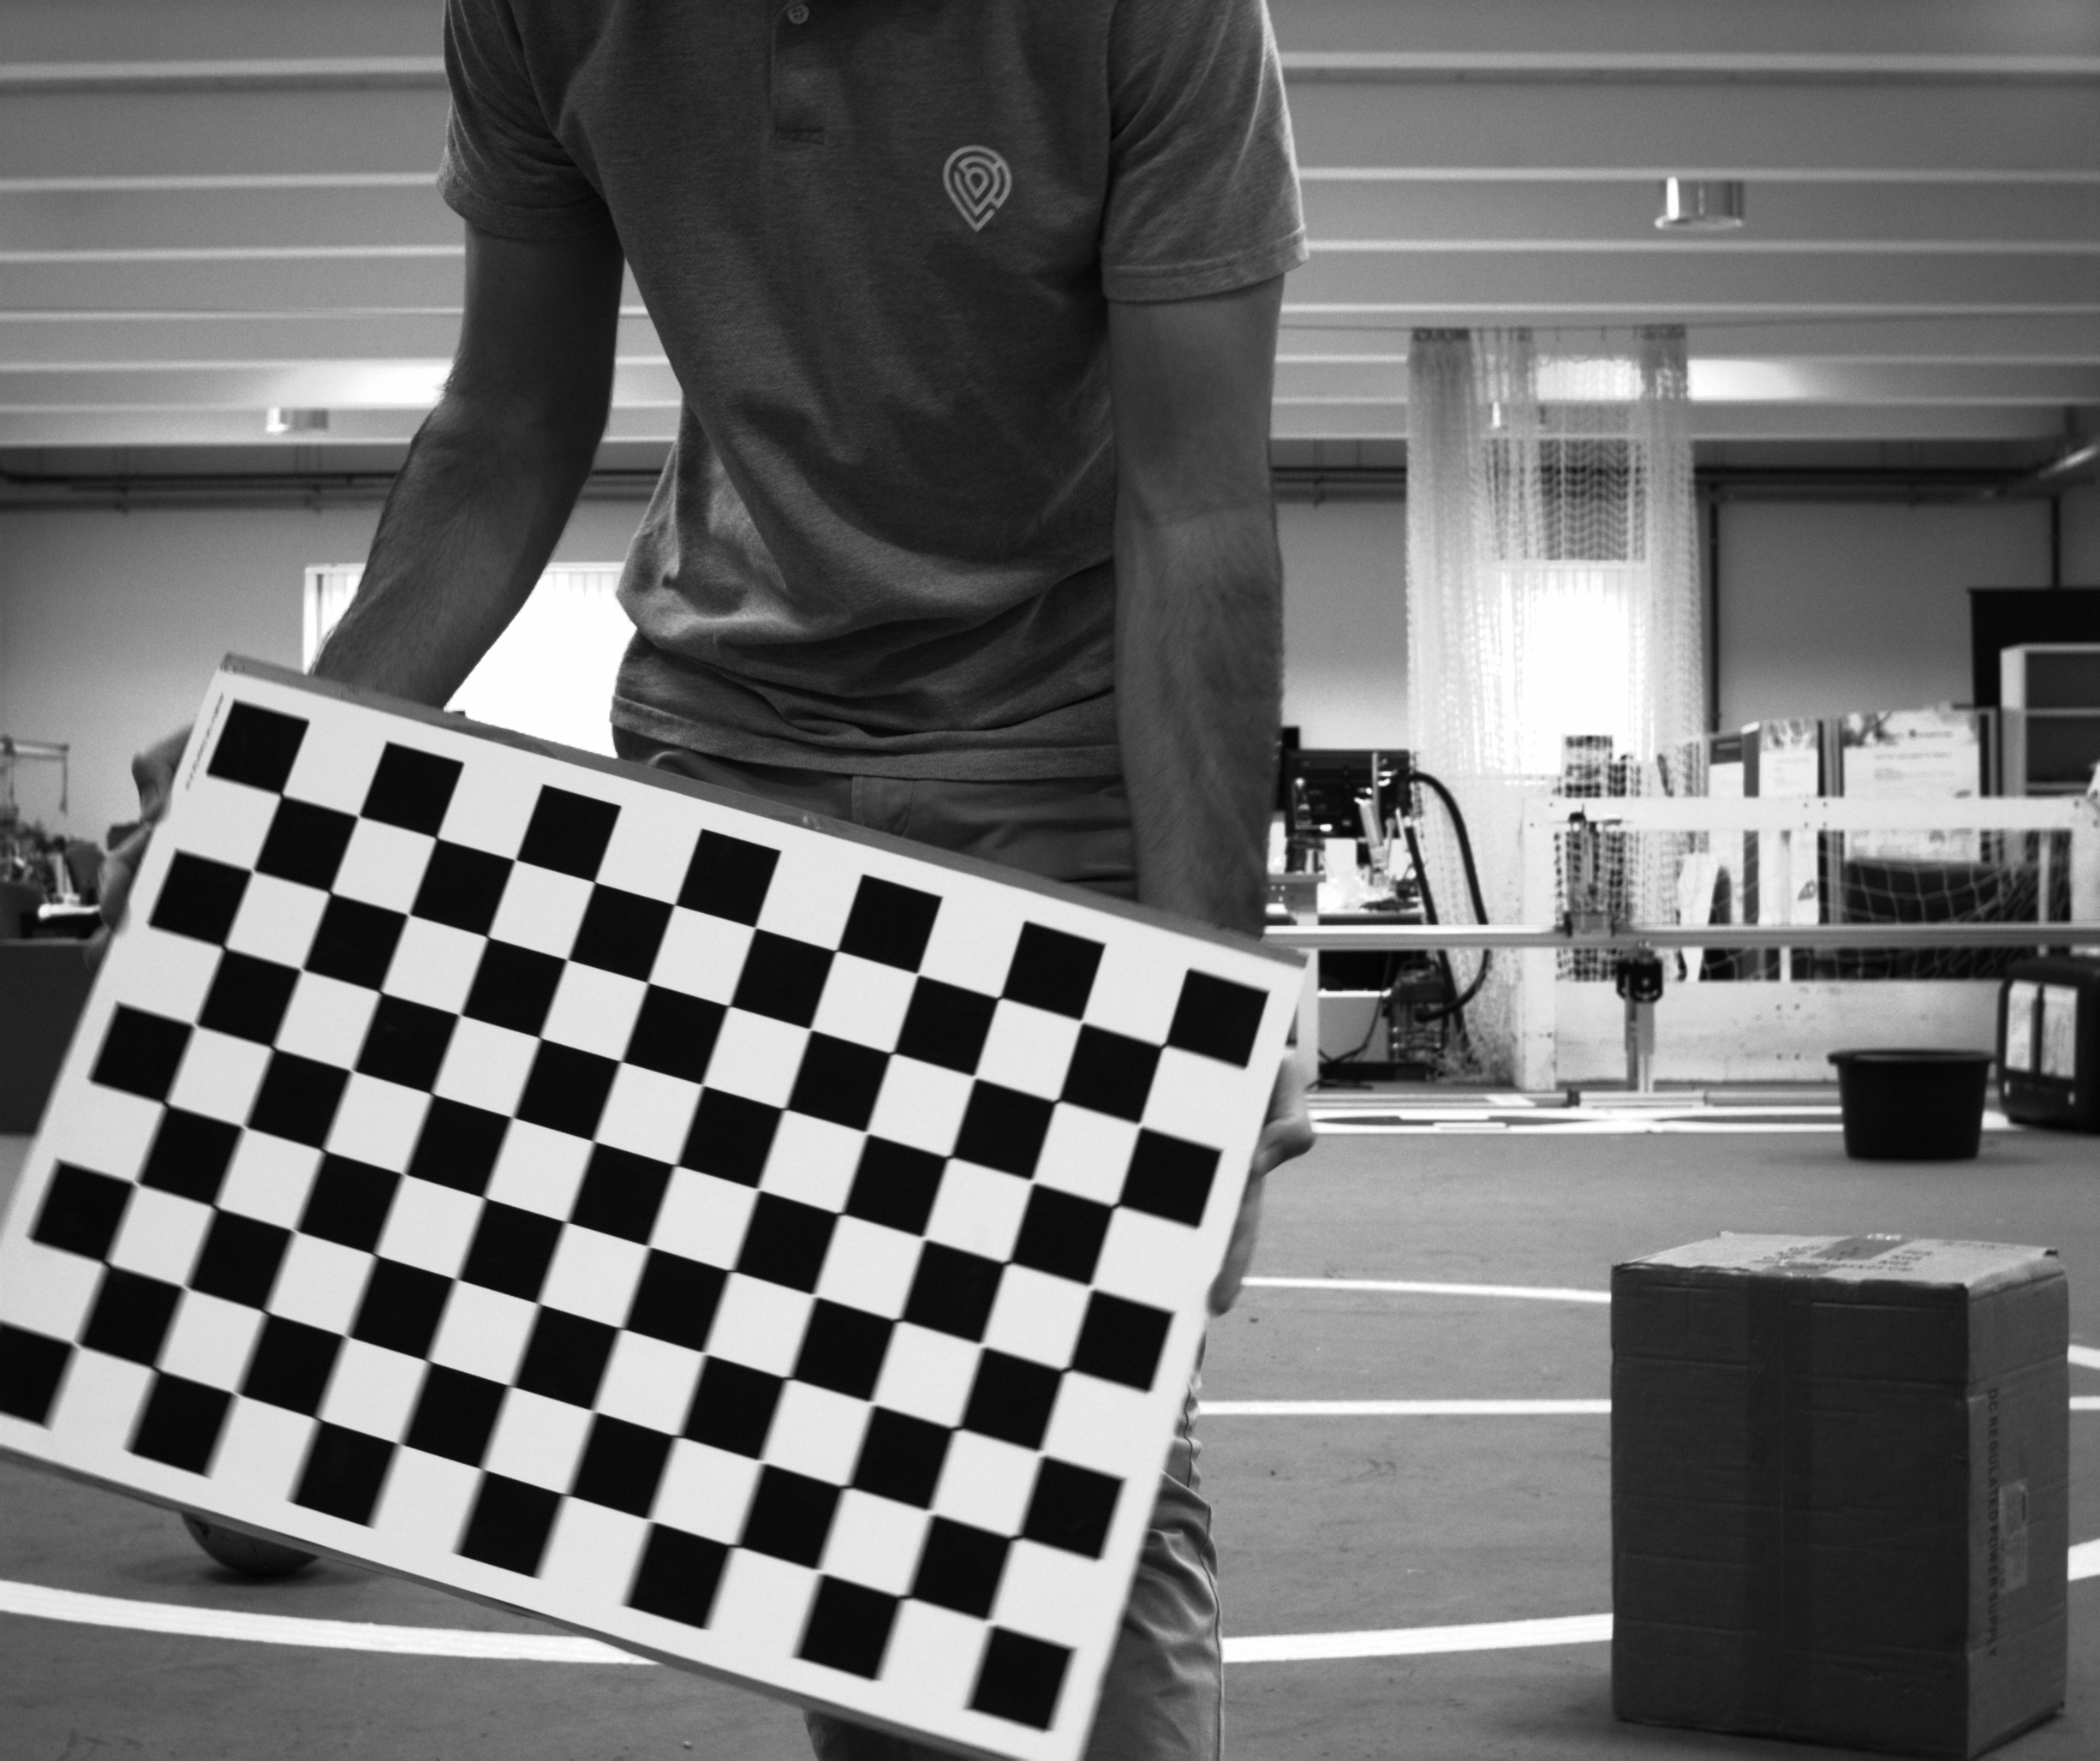
\includegraphics[width=0.9\textwidth]{img/camera-calibration/left-0044.png}
	\end{subfigure}
	\begin{subfigure}[c]{0.30\textwidth}
		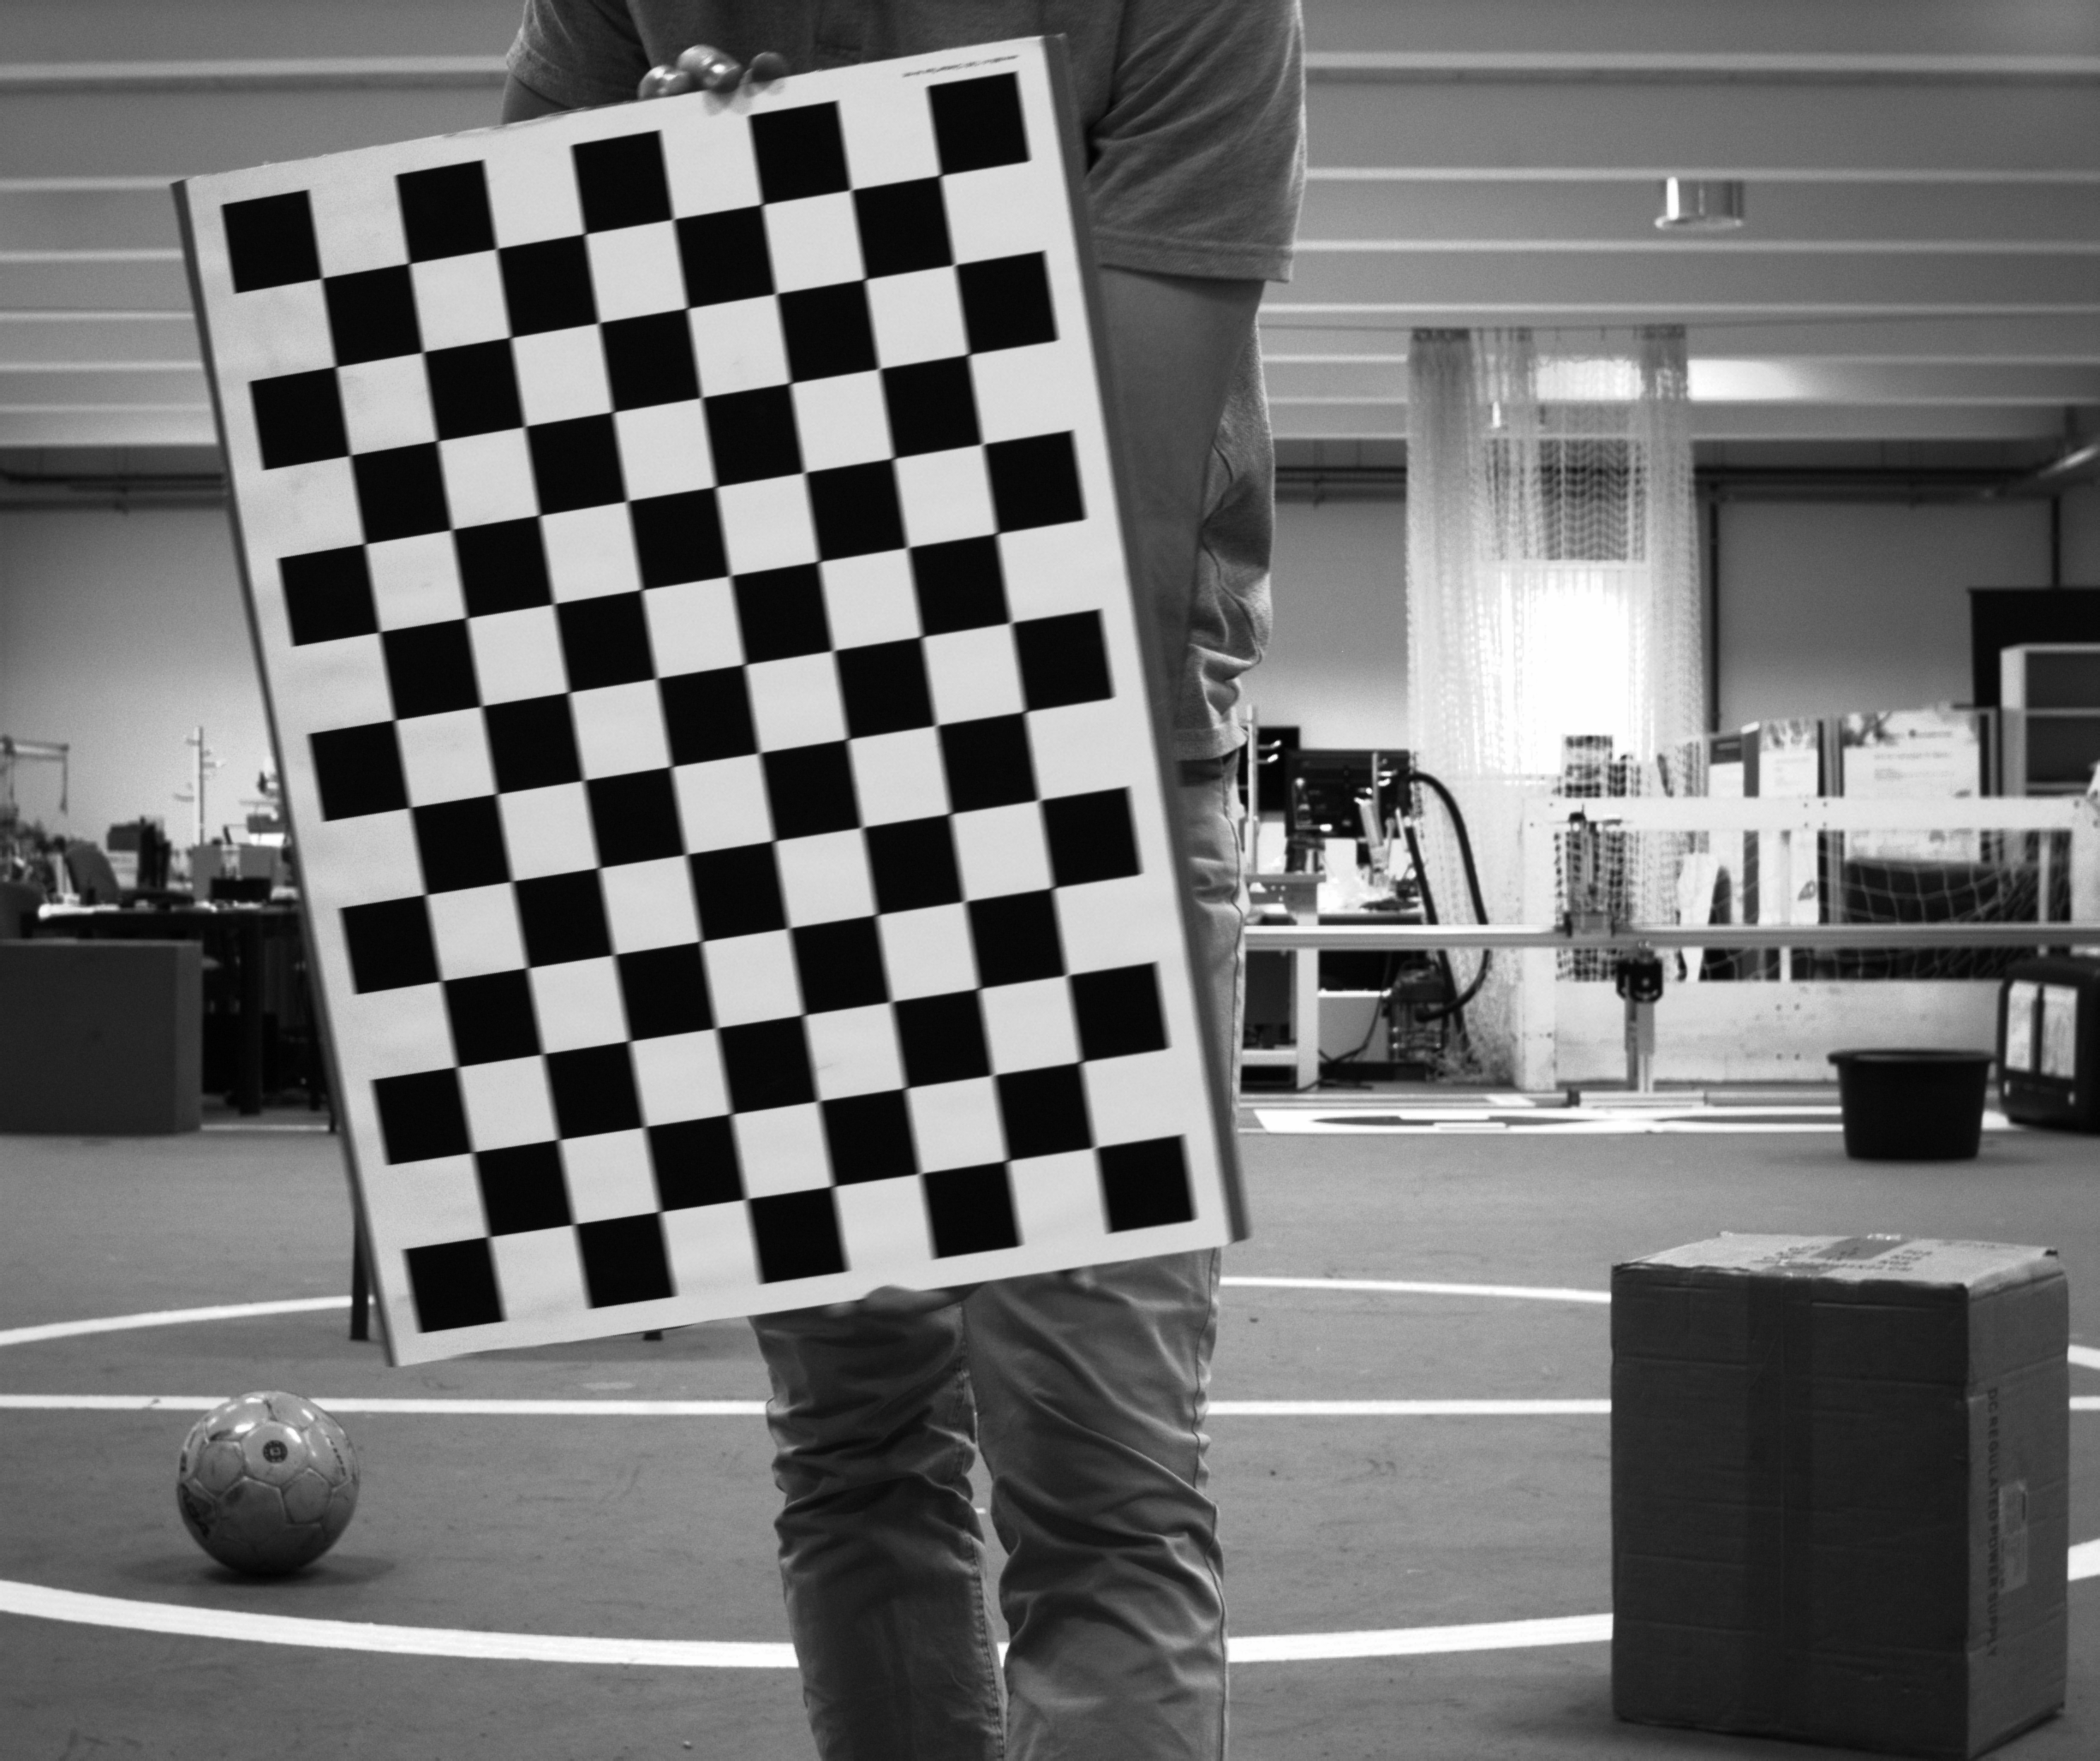
\includegraphics[width=0.9\textwidth]{img/camera-calibration/left-0048.png}
	\end{subfigure}
	
	\caption{Subset of 6 figures used on camera intrinsic calibration. The figures are all on greyscale and for each figure, the chessboard pattern was moved to generate an unique rotational matrix and translation vector in relation to the camera coordinate frame.}
	\label{fig:camera-calibration-images}
\end{figure}

\subsubsection{Frame Rate and Bandwidth concerns}
Despite the straightforwardness of the process, one of the secondary goals of this thesis is to produce a dataset of scenarios on which \ac{lidar} interference is present. Such goal implies that all data must be properly recorded, organized and stored, including calibration data. \ac{ros} provides \emph{rosbag}, a package for recording and playing back messages exchanged in a \ac{ros} network, which is used to save data on an external hard-drive.

However, preliminary tests with this tool indicate that it cannot save images topics at $9.2$~\ac{fps}. Other tests have shown that $8$~\ac{fps} is the best scenario where \emph{rosbag} can record data without causing buffer flush due to overrun errors. 

When calibrating the camera, \emph{camera\_calibration} package drops the frame rate to $\approx 4$~\ac{fps}, because it cannot operate at the desired data flow. If de-Bayerization and/or rectification is being applied to the image with intuit to save a pre-processed image, frame rate drops to $\approx 2$~\ac{fps}, since \emph{image\_proc}, the package responsible for pre-processing the image, cannot process images at the data-rate required for them to be saved on disk, introducing an overhead. Therefore, all images are sent from camera on the raw format \emph{BayerGB8} and recorded with \emph{rosbag} in the same format. Note that despite the camera providing  the \emph{RGB8Packed} color format, the hardware processing required on the camera hardware forces frame rate to be below $8$ \ac{fps}, reason why it was not chosen.

At 8~\ac{fps}, the bandwidth occupied by a 5~\ac{mp} image stream is $8 \cdot 2452 \cdot 2056 \approx 40 \text{Mbytes/s}$. Manta bandwidth limit configuration register was set to a value $25\%$ higher, to accommodate other transmissions from the computer to camera and vice-versa: $50$ Mbytes/s. No bandwidth problems were registered, only occasionally frame drops on the starting or ending of computer processes.

Therefore, for normal operation, Manta \ac{avt} G-504C is set to trigger image capture at a fixed frame rate of $8$~\ac{fps} and when being under an internal calibration procedure, at $4$~\ac{fps}. However, to run at this \ac{fps}, the camera must be able to output data at this speed, which is affected by other parameters.

\subsubsection{Lens Aperture and Exposure Time}
Thorlabs\cp~MVL16M1 lens has several possible apertures: $f/1.4$, $f/2.0$, $f/2.8$, $f/4.0$, $f/8.0$, $f/16.0$. The smaller the F-number\footnote{F-number represents the ratio of the lens' focal length to its diameter.}, the bigger the aperture and wider the lens entrance, allowing the camera sensor to be exposed to more light on the same time interval. More light indicates that exposure time can be reduced, since for the sensor to receive the same amount of light to produce a sharp image, less time is required to have passed from the starting of the exposition.

However, decreasing the F-number reduces the Hyperfocal distance (see equation~\ref{eq:hyperfocal_distance}), which in turns reduces \acf{dof}. A trade-off must then be addressed between \ac{dof} and F-number, which implies that three parameters must be fine-tuned: \ac{dof}, exposure time, image \ac{fps}, since they are all interconnected. As stated above, a maximum \ac{fps} is desirable, but due to recording constraints of the \emph{rosbag} package, $8$~\ac{fps} is the target image frame-rate. This implies that, at $8$\ac{fps}, the camera must never take more than $125ms$ since the start of exposure to the broadcast of the message on the Ethernet network, which means that exposure time must be inferior. Trough experimental analysis, the maximum exposure which seems to not disturb the desired frame rate is $100ms$. 

The F-number needs to be adjusted not only to ensure the requirements of the exposure time are met and to maximize \acl{dof}, but also to ensure that exposure can be increased or decrease to accommodate the daylight intensity variations. Such constrains result on a F-number of $f/4.0$ and an exposure time variation between $80ms$ to $100ms$ during daylight.

\subsubsection{\acl{dof} and calibration object}
Solving equation~\ref{eq:hyperfocal_distance} and replacing its result on equation~\ref{eq:dof-subject-distance}, we can obtain $d$, the object distance at each the camera must be focused. The object to be focused is the calibrating pattern and the $DoF_{near}$ limit is select to be the distance at which the calibration pattern fills the camera~\ac{fov}. The calculations can be seen on equation~\ref{eq:hyperfocal-and-dof-values}.

\begin{subequations}
	\label{eq:hyperfocal-and-dof-values}
	\begin{align}
		H & = \frac{16mm^2}{4.0 \cdot 0.020mm} + 16mm  = 3.216 m \label{eq:hyperfocal-distance-value} \\
		\vspace{25mm}
		d & = \frac{(3.216 - 16mm) \cdot 1.405}{3.216 - 1.405} = 2.49m \label{eq:dof-subject-distance-value}
	\end{align}
\end{subequations}

After focusing the camera, the \emph{cameracalibrator.py} node is run, using the command below. Note that the chessboard dimensions argument is $12\times 8$ and not $13 \times 9$, because the size argument refers to the number of interior corners, not number of squares.


\begin{verbatim}
    rosrun camera_calibration cameracalibrator.py --size 12x8 --square 0.044  
        monocular:=/camera image:=/camera/image_raw
\end{verbatim}


After the \ac{gui} registers all the images, the calibration parameters calculation can be initiated and the parameters are saved on a \textit{.ost} file for later use and/or sent the configuration to the camera. 

To interact with the Manta AVT G-504C, \emph{avt\_vimba\_camera} \ac{ros} package~\cite{AVTROSdriver}, which depends on VIMBA GigE SDK, is used to operate the camera. The package also provides compatibility with the \emph{camera\_calibration} package, crucial for a straightforward calibration process.

\subsection{Camera Calibration Results}
The \ac{ros} node diagrams can be seen on figure~\ref{fig:camera-calibration-rosgraph}. On sub-figure~\subref{fig:camera-calibration-avt-rosgraph}, the nodes and topics for the calibration procedure using the data directly from the driver are shown. Sub-figure~\subref{fig:camera-calibration-bag-rosgraph} shows the node graph if the data is being published by the \emph{rosbag} tool.


\begin{figure}[H]
	\vspace{5mm}
	\centering
	\begin{subfigure}[c]{0.8\textwidth}
		\centering
		\def\svgwidth{\columnwidth}
		\graphicspath{{img/camera-calibration/}}
		\includesvg{img/camera-calibration/bag-rosgraph}
		%
\includegraphics[width=0.8\textwidth]{img/camera-calibration/bag-rosgraph.png}
		\caption{\ac{ros} node graph for the camera calibration procedure using the \emph{rosbag} tool. \emph{RosbagPlayer} is the node that plays back the data stored on the bag file.}
		\label{fig:camera-calibration-bag-rosgraph}
	\end{subfigure}
	\vspace{5mm} \\ 
	\begin{subfigure}[c]{0.8\textwidth}
		\centering
		\def\svgwidth{\columnwidth}
		\graphicspath{{img/camera-calibration/}}
		\includesvg{img/camera-calibration/avt-rosgraph}
		%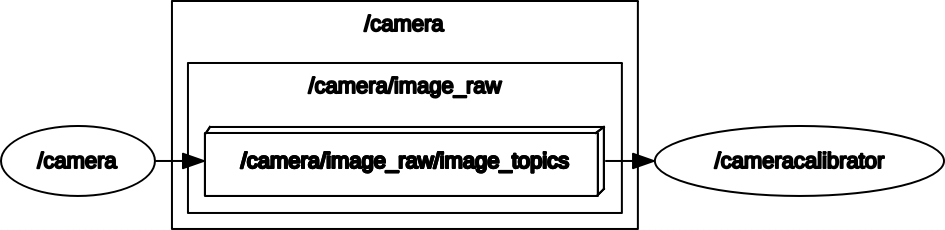
\includegraphics[width=0.8\textwidth]{img/camera-calibration/avt-rosgraph.png}		
		\caption{\ac{ros} node for the camera calibration procedure using the \ac{avt} Vimba \ac{ros} driver. \emph{camera} node refers to \ac{ros} node that wraps the \ac{avt} Vimba driver.}
		\label{fig:camera-calibration-avt-rosgraph}
	\end{subfigure}
	\caption{Camera Calibration node graph for \ac{ros} nodes. \emph{cameracalibrator} is the node responsible for computing the intrinsic camera calibration parameters, either if they are coming from the camera driver~\subref{fig:camera-calibration-avt-rosgraph} or the being replayed using \emph{rosbag}~\subref{fig:camera-calibration-bag-rosgraph}.}
	\label{fig:camera-calibration-rosgraph}
\end{figure}

The camera was calibrated everyday experimental measures were taken. The calibration for one of these days is shown below, on equation~\ref{eq:camera-calibration-results}.

\begin{subequations}
	\label{eq:camera-calibration-results}
	\begin{align}
		K & = 
		\begin{bmatrix}
			4595.944192 & 0.0         &  1313.9194945 \\
			0.0         & 4593.466666 &  952.554450 \\
			0.0         & 0.0         &  1.0
		\end{bmatrix} \\
		D & = 
		\begin{bmatrix}
			-0.304037 & 1.364428 &  -0.005705 & 0.003330 & 0.000000
		\end{bmatrix} \\
		P & = 
		\begin{bmatrix}
			4529.381836 & 0.0         & 1318.010062 & 0.0 \\
			0.0         & 4534.939941 & 947.167736  & 0.0 \\
			0.0         & 0.0         & 1.0         & 0.0 
		\end{bmatrix}
	\end{align}
\end{subequations}

	

\section{\ac{lidar} Intrinsic Calibration}
Unlike the camera, \acp{lidar} does not possess a typical calibration procedure. For Velodyne VLP-16 reflectivity measurements are factory calibrated, in a procedure described in~\cite{vlp16} and a \ac{xml} file is provided with the \ac{lidar}, containing corrections for the \ac{lidar} operating parameters.

This file must be converted to a more suitable format, \acs{yaml}~\footnote{\acs{yaml} is an acronym for \acl{yaml}. The author chose not to follow the norm of expanding acronyms' inline due to such  ``peculiar'' acronym, to facilitate reading.}, which is \ac{ros} default and can be loaded by the Velodyne \ac{ros} driver package, \emph{velodyne}, for correction of the \ac{lidar} measurements. After observing the point cloud with tests objects such as boxes and walls, \ac{lidar} calibration is concluded to be accurate and no further procedures were undertaken.

\section{Camera and \ac{lidar} Extrinsic Calibration}
\label{sec:calibration:extrinsic}
Calibrating the camera and \ac{lidar}, as explained in section~\ref{subsec:sota:camera-intrinisc-calibration}, requires determining the rigid body transform between the reference frames of the two sensors. A rigid body transform, also known as an Euclidean Isometry since it preserves the distance between points~\cite{mvg_book}, has 6 \ac{degof}, that can be represented by a translation and a rotation vector.

Due to the ambiguity of the rotation vector and its variety of interpretations: it can represent one of twelve Euler angles notation, angle axis notation, amongst others; this notation is normally replaced by the unambiguous rotation matrix (see equation~\ref{eq:camera_transform_full} for an example) or a quaternion. Such representations are also free from gimbal lock, a mathematical limitation of the vector representation, that can cause one rotation axis ``locking'' on another, resulting on their rotation no longer being independent of the other, removing one \ac{degof} and degenerating into a two-dimensional rotational space. For more details on gimbal lock and other singularities see~\cite{mvg_book, Slabaugh, camera_models}.

On this thesis, the preferred notation is a quaternion, which is also adopted by \ac{ros}~\cite{Foote2014}. A quaternion is a mathematical object belonging to $\mathbb{R}^4$, that has a vector (or imaginary) part and a scalar (or real) part. Its representation is denoted on equation~\ref{eq:quaternion-notation}, where $\mathbf{i}$, $\mathbf{j}$ and $\mathbf{k}$ are the normalized unit vectors of the $x$, $y$ and $z$ axis, respectively; and $w$ is the scalar part. More information on quaternions can be found on~\cite{mvg_book}.

\begin{equation}
	\label{eq:quaternion-notation}
	q = (x\mathbf{i}, y\mathbf{j}, z\mathbf{k}, w)
\end{equation}

\subsection{Calibration Method}
Given the nature of the sensors: a camera image is two-dimensional and the \ac{lidar} data is tridimensional; the extrinsic calibration needs to consider the projective geometry and its transformations on the camera. Revisiting equation~\ref{eq:jointRotationTranslationTransform}, our goal is to determine the joint rotation and translation matrix that allows the conversion of coordinates from the \ac{lidar} to the camera frame. To account for projective geometry, equation~\ref{eq:camera_transform_full} must be considered when establishing 3D points to image pixels correspondences.

The method implemented to calibrate the camera and \ac{lidar} is inspired by Scaramuzza~\etal~\cite{Scaramuzza} and Brabec's~\cite{brabec2014} work. The method proposed consists on manually selecting the correspondences between the image pixels and the 3D points on the \ac{lidar} point cloud. If a single synchronized frame from the camera and \ac{lidar} is used, one can consider the scene as static, and therefore, the joint rotation and translation matrix present in equation~\ref{eq:camera_transform_full} is actually the same as the matrix present on~\ref{eq:jointRotationTranslationTransform}. 

Such considerations are only possible do to the camera using a Global Shutter instead of rolling shutter. On the former, the image is acquired on a single shot and all the points ``have the same timestamps''. On the latter, each row of the image is acquired iteratively, therefore, ``having different timestamps''. If a rolling shutter camera was used, for a single image the \ac{lidar} point cloud could not have been considered static and the delays on the camera shutter and \ac{lidar} rotation must be accounted when calibrating and fusing the data between the two.

Since the intrinsic calibration matrix is already obtained by the method described on section~\ref{sec:calibration:camera}, and the correspondences are selected by the user, the only unknown remaining is the joint rotation and translation matrix. Also, since this method ``reuses'' the equations that are the basis for intrinsic camera calibration, it can also ``reuse'', with some constraints and modifications, the same algorithms~\cite{opencv_doc}.


\subsection{Implementation}
To extrinsically calibrate the camera and \ac{lidar}, a multi-node network approach was followed, which can be seen on figure~\ref{fig:extrinsic-calibration-rosgraph}. Using \ac{opencv} and \ac{pcl}, two visualizers were encapsulated under \ac{ros} nodes written in C++, that subscribe camera and \ac{lidar} messages, respectively. The point cloud visualizer, \emph{PCL\_Viewer\_with\_Pose}, receives the point cloud data from the \emph{rosbag} player or the \emph{velodyne} driver and publishes the coordinates of the selected point and the viewer pose. \emph{Image\_Visualizer} publishes the pixels selected by the user, but requires the de-Bayering and conversion to RGB of the raw image using the \emph{image\_proc} package. Despite being wrapped in \ac{ros}, each of the visualizers provides standalone callbacks, that support ``frame freezing'' for correspondences selection.

Another node, \emph{rigid\_transform\_computation} is responsible for listening to messages containing the selected pixels and points, registering their correspondences. This node  instantiates two \ac{ros} services servers, that can be called asynchronously: one for computing the rigid body transform and another to save the correspondences selected on a \ac{csv} file, for later usage. 

\begin{figure}[ht]
	\centering
	\def\svgwidth{\columnwidth}
	\graphicspath{{img/calibration/}}
	\includesvg{img/calibration/extrinsic-calibration-rosgraph}
	\caption{\ac{ros} node graph for the extrinsic calibration. The nodes are represented on  ellipses and the topics between them on rectangles. Rosbag Player is responsible reproducing the recorded topics.}
	\label{fig:extrinsic-calibration-rosgraph}
\end{figure}


The algorithm implemented to compute the 6-\ac{degof} rigid body transform uses \ac{opencv} \emph{solvePnP}, that given the intrinsic camera parameters and the correspondences between the object points (3D points from \ac{lidar}), computes the rotation and translation vectors. For solving the \ac{pnp} problem, several algorithms can be used: Levenberg-Marquardt~\cite{Levenberg1943}, Effective~\ac{pnp}~\cite{Lepetit2009}, Perspective-Three-Point~\cite{Gao2003}, Direct-Least-Squares~\cite{Hesch2011} or Exhaustive Linearization — Uncalibrated \ac{pnp}~\cite{Penate-Sanchez2013a}. The \ac{ros} node implemented provides an argument to select the desired algorithm to be applied to solve the \ac{pnp} problem.

After resolving the \ac{pnp} with one of the methods above, Rodrigues' algorithm is used to convert the \ac{opencv} rotation vector to a rotation matrix~\cite{Dai2015}, which is then used to construct the quaternion. Combining the quaternion with the translation vector, a static transform is published to the \ac{ros} network, which can be used to convert and fuse data from the camera coordinate frame to the \ac{lidar} and vice-versa.

Additional nodes are also created to load the correspondences between the 3D points and image pixels from the \ac{csv} file and the camera intrinsic parameters from an \ac{yaml} file, compute the rigid body transform and publish it under a \ac{ros} static transform node, for usage in a \ac{ros} network.


\subsection{Calibration Result}
To ease the calibration file, a \ac{ros} launch file is created. A launch file is written in \ac{xml} and provides the  \ac{ros} master instructions on how to run all the necessary nodes to implement a desired functionality. On this case, \emph{rigid\_transform\_computation.launch}, launches the two visualizers and the node responsible for listening to the selected correspondences. 

Several tests were performed with the possible algorithms for solving \ac{pnp}. Since for the version of \ac{opencv} used, $3.2.0$, the Direct-Least-Squares and Uncalibrated \ac{pnp} methods are unstable\cite{opencv_doc}, only the Levenberg-Marquardt, Perspective-Three-Point and Effective~\ac{pnp} were tested. 

Despite the extrinsic calibration scenario using the planar chessboard present on the camera intrinsic calibration procedure, the algorithm implemented does not require the usage of a calibration object. For calibration, 6 points were selected on the point cloud and six pixels on the image: 4 correspond to the corners of the chessboard and two to a background object. The selected correspondences can be seen on figure~\ref{fig:calibration-correspondences}: sub figure~\subref{fig:extrinsic-calibration-correspondences:camera} shows the selected pixels on the image, marked with red crosses; sub figure~\subref{fig:extrinsic-calibration-correspondences:lidar} shows the selected 3D points on the point cloud, marked as red spheres.


\begin{figure}[H]
	\centering
	\begin{subfigure}[c]{0.39\textwidth}
		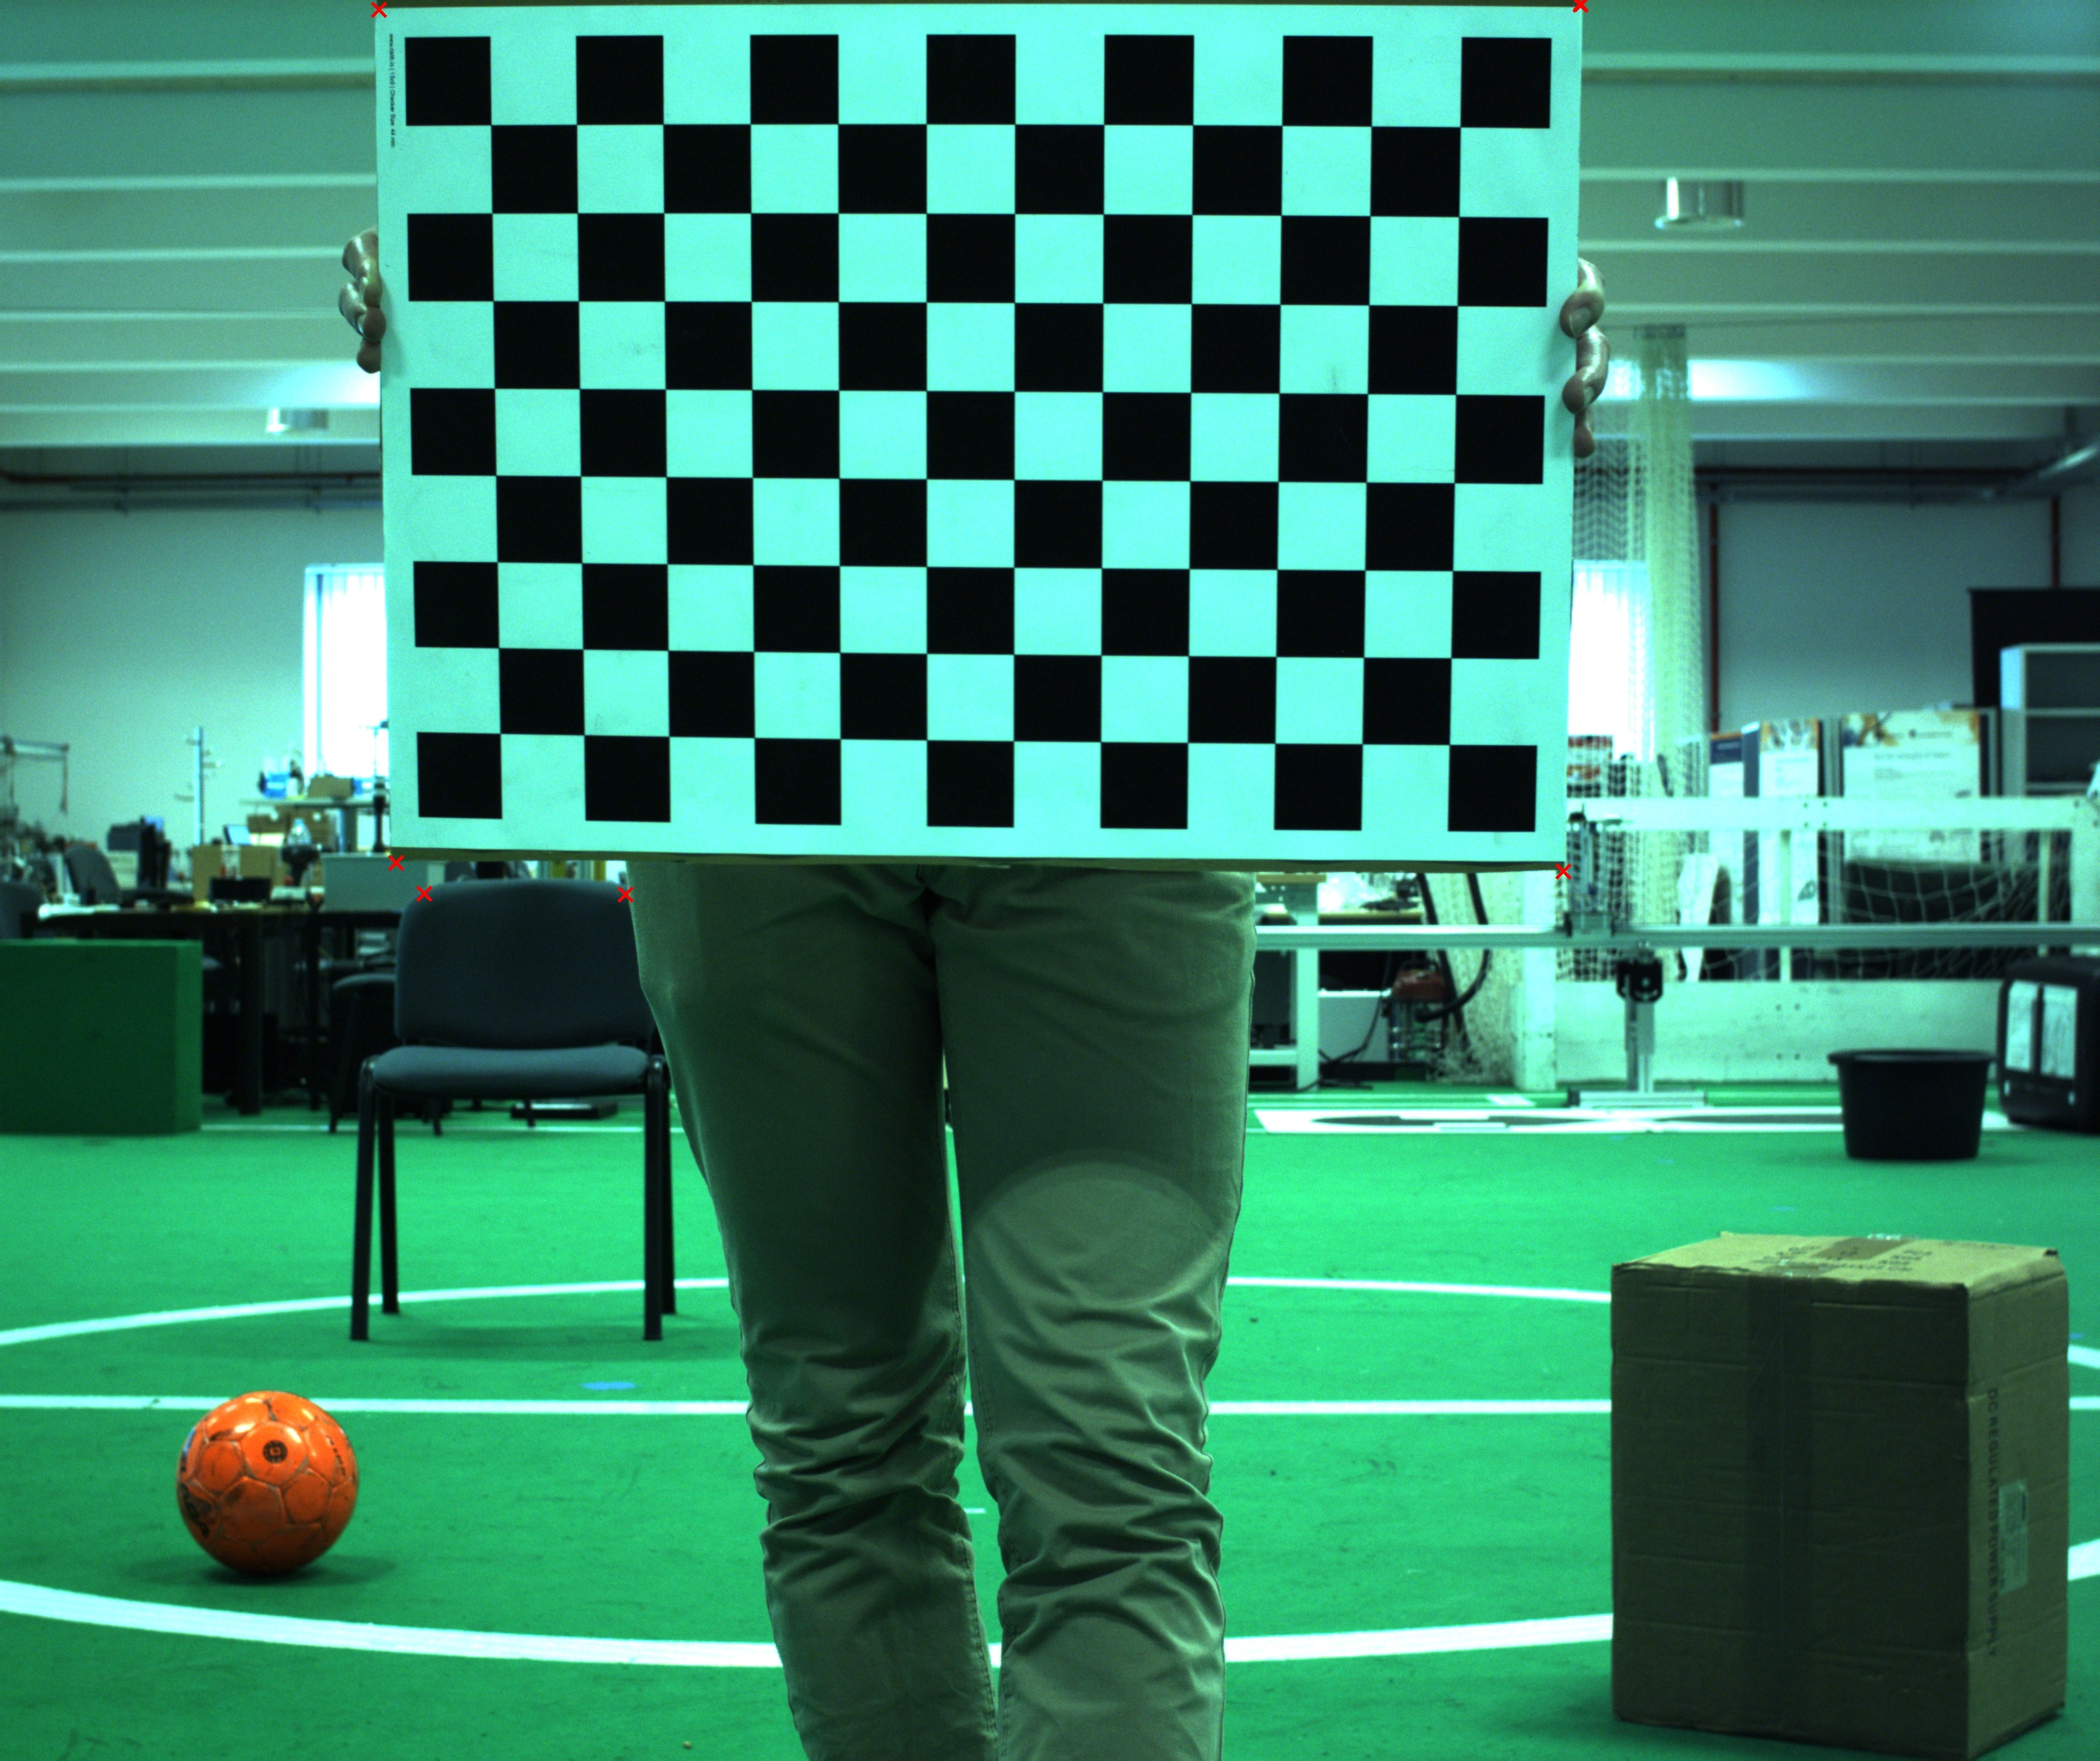
\includegraphics[width=\textwidth]{img/calibration/camera-extrinsic-calibration-points.jpg}
		\caption{Image used on the extrinsic calibration procedure. The selected pixels are marked with a red cross.}
		\label{fig:extrinsic-calibration-correspondences:camera}
	\end{subfigure}
	\qquad
	\begin{subfigure}[c]{0.55\textwidth}
		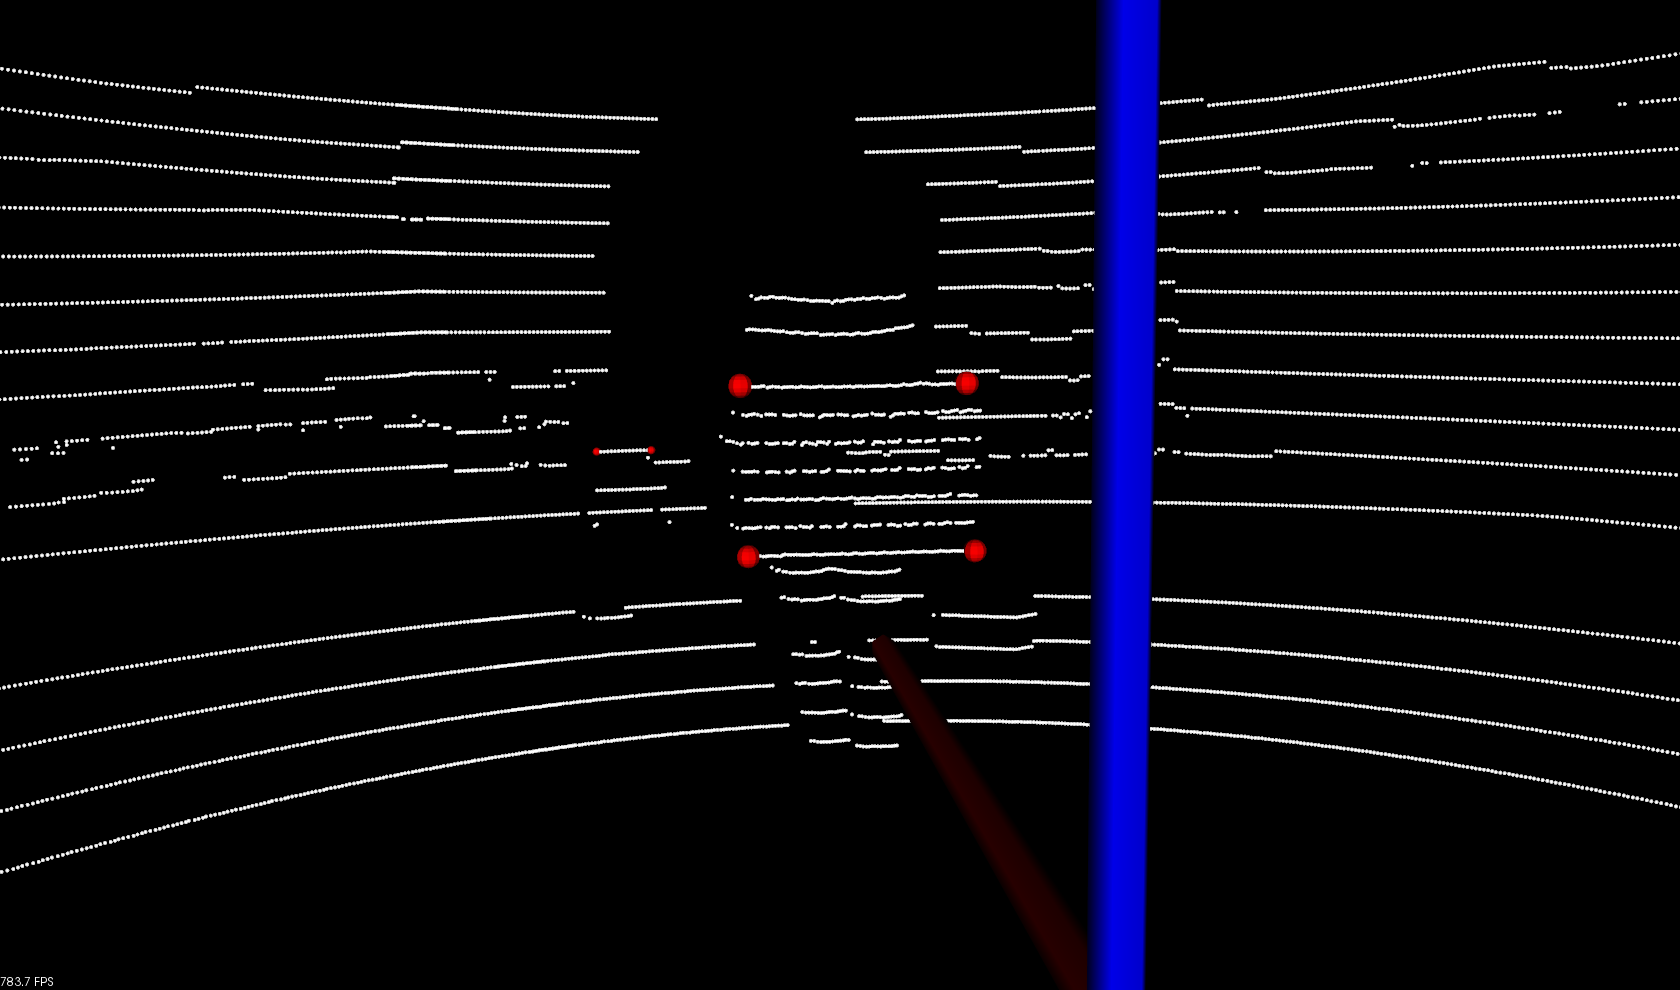
\includegraphics[width=\textwidth]{img/calibration/lidar-extrinsic-calibration-points.png}
		\caption{Region of the point cloud containing the correspondences used on the extrinsic calibration procedure. The selected 3D points are marked with a red sphere.}
		\label{fig:extrinsic-calibration-correspondences:lidar}
	\end{subfigure}
	\caption{Image and Region of the Point Cloud used on the extrinsically calibration between the camera and the \ac{lidar}. The correspondences are marked with red crosses or spheres, respectively, and correspond to the 4 corners of the chessboard and the limit of the chair on the background.}
	\label{fig:calibration-correspondences}
\end{figure}

After the computation, the rotation and translation is obtained from the camera frame to the \ac{lidar} frame. If the transformation from the \ac{lidar} to the camera frame is required, the inverse transformation can be obtained by inverting the scalar component of the quaternion, $w$, such as $w^{LiDAR}_{camera} = - w^{camera}_{LiDAR}$. 

Extrinsic camera and \ac{lidar} calibration was performed everyday  experimental measures were taken. The calibration for the camera intrinsic parameters given on equation~\ref{eq:camera-calibration-results} and the correspondences shown on image~\ref{fig:calibration-correspondences} are presented on equation~\ref{eq:camera-to-lidar-transform}. On figure~\ref{fig:extrinsic-calibration-frames}, a visualization of the experimental setup sensors coordinate frames and the transform between them is given.

\begin{subequations}
	\label{eq:camera-to-lidar-transform}
	\begin{align}
		t = \begin{bmatrix}
			-0.156714088124  \\
			-0.0206731034739 \\
			-0.258170823407
		\end{bmatrix}
		& \qquad
		q = \begin{bmatrix} 
		0.487219246678  \\
		-0.499909358687 \\
		0.521690432045  \\
		-0.490456044796
	\end{bmatrix}
	\end{align}
\end{subequations}

\begin{figure}[H]
	\centering
	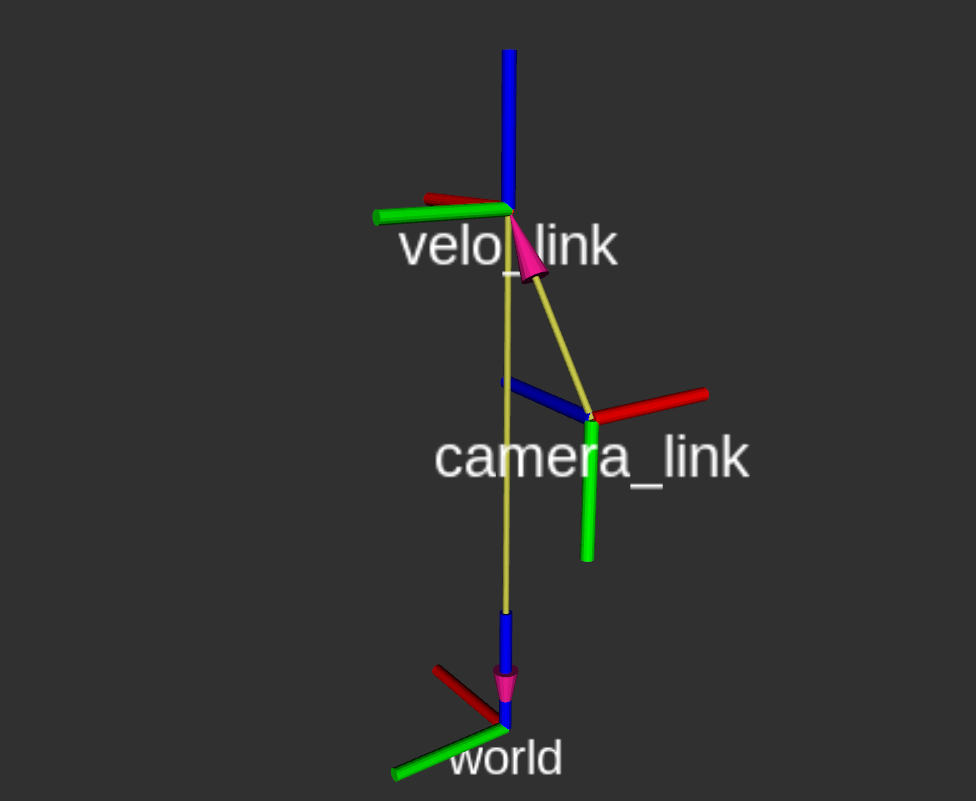
\includegraphics[width=0.6\textwidth]{img/calibration/extrinsic-calibration-frames.png}
	\caption{TF visualization of the relation between the experimental setup coordinate frames. \emph{velo\_link} and \emph{camera\_link} represent the coordinate frames of the Velodyne VLP-16 \ac{lidar} and the Manta \ac{avt} G-504C, respectively. The \emph{world} coordinate frame represents the positioning of the \ac{lidar} in the world, which in this case is an offset to the vertical positioning of the \ac{lidar}.}
	\label{fig:extrinsic-calibration-frames}
\end{figure}

